\documentclass[12pt,a4paper,openany]{report}

\usepackage[spanish,es-tabla,shorthands=off]{babel}
\usepackage[utf8]{inputenc}
\usepackage[T1]{fontenc}
\usepackage{lmodern}
\usepackage[margin=2.5cm]{geometry}
\usepackage{graphicx}
\graphicspath{{figuras/}}
\usepackage{float}
\usepackage{pdflscape}
\usepackage{booktabs}
\usepackage{longtable}
\usepackage{array}
\usepackage{enumitem}
\usepackage{listings}
\usepackage{amsmath}
\usepackage{xurl}
\usepackage{hyperref}

\hypersetup{
  colorlinks=true,
  linkcolor=black,
  urlcolor=blue,
  pdftitle={Borrador 1. Alineación entre contratos OpenAPI bancarios y modelos de referencia BIAN},
  pdfauthor={Alex Mancilla Antay y Dennis Jack Paitan Cano}
}

\renewcommand{\contentsname}{Índice de contenidos}
\renewcommand{\listtablename}{Lista de tablas}
\renewcommand{\listfigurename}{Lista de ilustraciones}
\renewcommand{\thechapter}{\Roman{chapter}}
\renewcommand{\thesection}{\arabic{chapter}.\arabic{section}}
\renewcommand{\thesubsection}{\arabic{chapter}.\arabic{section}.\arabic{subsection}}

\newcommand{\pendiente}{%
  \par\vspace{0.6em}
  \textit{Pendiente de redacción en este borrador.}\par}

\lstset{
  basicstyle=\ttfamily\small,
  breaklines=true,
  columns=fullflexible,
  frame=single,
  language=bash
}

\begin{document}

\begin{titlepage}
  \thispagestyle{empty}
  \centering

  \vspace*{0.4cm}
  {\Large\bfseries UNIVERSIDAD NACIONAL DE INGENIERÍA\par}
  \vspace{0.3cm}
  {\normalsize\bfseries UNIDAD DE POSGRADO FACULTAD DE INGENIERÍA DE SISTEMAS Y COMPUTACIÓN\par}
  {\normalsize\bfseries / ESCUELA DE POSGRADO\par}

  \vspace{0.7cm}
  
\includegraphics[width=3.2cm]{escudo-uni.png}
  \vspace{0.7cm}

  {\large\bfseries TESIS\par}
  \vspace{0.15cm}
  {\normalsize Borrador 1\par}
  \vspace{0.55cm}
  {\normalsize\bfseries ``ALINEACIÓN ENTRE CONTRATOS OPENAPI BANCARIOS Y MODELOS DE REFERENCIA BIAN\\
  MEDIANTE ANÁLISIS ESTRUCTURAL Y SIMILITUD SEMÁNTICA''\par}
  \vspace{1.0cm}

  {\normalsize PARA OBTENER EL GRADO ACADÉMICO DE\par}
  {\normalsize MAESTRO EN CIENCIAS CON MENCIÓN EN:\par}
  {\normalsize INTELIGENCIA ARTIFICIAL\par}
  \vspace{1.0cm}

  {\normalsize\bfseries ELABORADA POR:\par}
  \vspace{0.2cm}
  {\normalsize\bfseries ALEX MANCILLA ANTAY\par}
  {\normalsize\bfseries DENNIS JACK PAITAN CANO\par}
  \vspace{0.4cm}
  {\normalsize Grupo 10\par}
  \vspace{0.7cm}

  {\normalsize\bfseries ASESOR:\par}
  \vspace{0.2cm}
  {\normalsize\bfseries POR DESIGNAR\par}

  \vfill
  {\normalsize\bfseries LIMA, PERÚ\par}
  \vspace{0.25cm}
  {\normalsize\bfseries 2026\par}
\end{titlepage}

\chapter*{Datos generales}
\addcontentsline{toc}{chapter}{Datos generales}

\begin{enumerate}[leftmargin=1.4em]
  \item \textbf{Título de la tesis:} Alineación entre contratos OpenAPI bancarios y modelos de referencia BIAN mediante análisis estructural y similitud semántica.
  \item \textbf{Autores:} Alex Mancilla Antay; Dennis Jack Paitan Cano. Grupo 10.
  \item \textbf{Asesor:} Por designar.
  \item \textbf{Área:} Inteligencia artificial. Alineación de contratos OpenAPI bancarios con Service Domains BIAN.\\
        Unidad de Posgrado: Facultad de Ingeniería de Sistemas y Computación.\\
        Programa: Maestría en Inteligencia Artificial.
  \item \textbf{Lugar:} Universidad Nacional de Ingeniería, Lima, Perú.
  \item \textbf{Duración estimada:} 5 meses (septiembre 2026 -- enero 2027).
  \item \textbf{Estado de este archivo:} borrador 1, 21 de noviembre de 2026. Los capítulos que todavía no están redactados llevan el título y la marca de pendiente.
\end{enumerate}

\chapter*{Dedicatoria}
\addcontentsline{toc}{chapter}{Dedicatoria}
\pendiente

\chapter*{Agradecimientos}
\addcontentsline{toc}{chapter}{Agradecimientos}
\pendiente

\chapter*{Copia de documentos}
\addcontentsline{toc}{chapter}{Copia de documentos}
\pendiente

\tableofcontents

\listoftables
\addcontentsline{toc}{chapter}{Lista de tablas}

\listoffigures
\addcontentsline{toc}{chapter}{Lista de ilustraciones}

\chapter*{Resumen}
\addcontentsline{toc}{chapter}{Resumen}

% REESCRIBIR A MANO POR ALEX Y JACK
% Borrador, no cerrado. En el plan, esta página salió casi entera en el reporte del 30 %.
% Léanlo en voz alta y cambien cualquier frase que no dirían en la sustentación.

Queremos saber, antes de integrar, si el YAML de una API bancaria cuenta el mismo negocio que el Service Domain BIAN con el que se lo empareja. Hoy eso se mira a ojo, o no se mira.

En la mesa abrimos el archivo y el dominio. Paths, el \texttt{operationId}, los \texttt{\$ref}. Si el contrato dice \texttt{paymentRequest} y el dominio dice \texttt{PaymentOrder}, no queda un número. Sobre esa instancia calculamos S, E y C, y los tres entran en el AlignmentScore.

El 6 de noviembre de 2026 el parser firmó 296 de 296 YAML: 38 de Open Finance Brasil y 258 de BIAN v14. En I1 a I6 el S léxico quedó entre 0,00 y 0,03. MiniLM, sin ajuste nuestro, mueve cinco de esas siete de Nula a Baja. I4 se queda en Nula. I6, enrollments contra Payment Order Initiation, se queda en cero. Reino Unido, Berlin Group, STET y el resto de la lista pública no tienen score en este borrador.

Lo que no entra ---banco emisor, 38$\times$258, el F1--- está en la sección de alcances.

\vspace{0.4cm}
\noindent\textbf{Palabras clave:} OpenAPI; BIAN; AlignmentScore; schema matching; API bancaria; alineación estructural.

\chapter*{Abstract}
\addcontentsline{toc}{chapter}{Abstract}

% REESCRIBIR A MANO POR ALEX Y JACK
% Draft, not closed. Do not treat this as a translation of the Spanish summary.
% Read it aloud and replace any sentence you would not say in the defense.

On 6 November 2026 the parser signed 38 Open Finance Brasil YAML files and 258 BIAN v14 domains, 296 of 296. Lexical S on I1--I6 sits between 0.00 and 0.03. The score we report is the cosine of paraphrase-multilingual-MiniLM-L12-v2, pretrained, not fine-tuned. I1, I2, I3a, I3b and I5 move from Nula to Baja. I4 stays Nula, at 0.35. I6, enrollments against Payment Order Initiation, stays at 0. UK Read/Write, the Berlin Group, STET, PolishAPI, the Czech standard, Australia, Payments NZ, Bahrain and the Nebras YAML are in the corpus. They have no score here. An issuing-bank file, the full 38$\times$258 cross-product and an F1 are out.

\vspace{0.4cm}
\noindent\textbf{Keywords:} OpenAPI; BIAN; AlignmentScore; schema matching; banking API; structural alignment.

\chapter*{Introducción}
\addcontentsline{toc}{chapter}{Introducción}

El cruce entre el contrato que publica el banco y el Service Domain que usa el arquitecto se hace a ojo, o no se hace. El archivo trae paths, el verbo, el operationId y los \$ref. El dominio trae behaviors y objetos de negocio. Si uno dice \texttt{paymentRequest} y el otro \texttt{PaymentOrder}, no queda un número en el expediente.

Ese número es el AlignmentScore. Sale de tres piezas: parecido de significado (S), correspondencia de la jerarquía REST (E) y cobertura de los conceptos del dominio (C). El objeto sigue siendo el contrato OpenAPI bancario. Open Finance Brasil es la parte del corpus que ya corrimos. Reino Unido, Berlin Group, STET, PolishAPI, Chequia, Australia, Nueva Zelanda, Baréin y Emiratos entran al mismo procedimiento y, en este borrador, todavía no tienen score.

Los capítulos I y II fijan el objeto y de dónde sale cada score. El III trae I1 a I6. El IV no estira esas siete instancias al resto del corpus.

\chapter{Planteamiento del problema}

\section{Diagnóstico}

Los síntomas están en el sector, no en la matriz. En 2018 la migración de plataformas del TSB dejó sin servicio a cerca de 1,9 millones de clientes. Los informes públicos hablan de cientos de millones de libras y de semanas con la operación restringida \cite{UKTreasuryTSB2018}. Ese expediente no nombra OpenAPI ni BIAN. Muestra otra cosa: el negocio y la plataforma se movieron sin una correspondencia que se pudiera verificar.

El \textit{open banking} deja el caso más seco. Desde 2018 la regulación británica obligó a nueve bancos de \textit{retail} a exponer APIs \cite{CMA2016}. Publicar el Swagger no acerca esas interfaces a un modelo de negocio de referencia. Eso se sigue resolviendo en la mesa.

Casas et al.\ \cite{Casas2021} mapearon 47 estudios primarios. Solo el 40\,\% ancla un dominio concreto. El 68\,\% propone herramientas y el 43\,\% mejora la documentación. Golmohammadi et al.\ \cite{Golmohammadi2024}, sobre 92 trabajos de prueba REST, subrayan el costo de validar servicios ya desplegados. Farzi \cite{Farzi2021} acerca BIAN a la agilidad bancaria y deja dicha la distancia entre el \textit{to-be} y lo que corre.

El 21 de noviembre de 2026 buscamos contratos bancarios que se puedan bajar sin cuenta. Aparecen, además de Open Finance Brasil, el Read/Write del Reino Unido (v4.0.1), el XS2A del Berlin Group (v1.3.16) y su openFinance, STET 1.6.3.2, PolishAPI 3.0, el estándar checo 9.0.0, el \textit{Consumer Data Right} australiano (banca 1.36.0), Payments NZ, el marco de Baréin y los YAML de Open Finance de Emiratos en el repositorio de Nebras. Son estándares de cuentas, pagos o ambos. Ninguno trae, en el propio archivo, un score contra un Service Domain BIAN.

\section{Identificación y descripción del problema de estudio}

El objeto no es un banco ni BIAN entero. Es el contrato OpenAPI 3.x con el que el sector describe la API. BIAN entra como modelo de referencia: Service Domains, con behaviors y business objects. La unidad de análisis es la operación del contrato frente al behavior o al objeto del dominio.

En el día a día el desajuste se ve en los nombres. El contrato dice \texttt{paymentRequest} y el dominio dice \texttt{PaymentOrder}. Un PUT del dominio no tiene GET en el YAML, o al revés. En Open Finance Brasil, \texttt{payments} 4.0.0 publica \texttt{POST /pix/payments}. En BIAN v14, Payment Order Initiation llama a esa acción \texttt{Initiate}. \texttt{enrollments} 2.1.0 da de alta un dispositivo (FIDO). No es una orden de pago. Emparejarlo a la fuerza con ese dominio no mide alineación.

BIAN también publica OpenAPI de sus dominios. No por eso medimos BIAN contra BIAN. El archivo que entra es el del estándar o del catálogo: \textit{paths}, \texttt{operationId} y \textit{schemas}. El dominio entra como negocio.

En el sprint, desarrollo publica el YAML. Arquitectura guarda el Service Domain. Un release mueve rutas y el modelo no se entera. La versión del archivo no apunta a una revisión del dominio.

Shabbir et al.\ \cite{Shabbir2025} recuerdan que la consistencia se resiente cuando la documentación técnica no refleja el dominio. La revisión, cuando existe, es una lectura humana o una herramienta genérica de \textit{schema matching} \cite{Shvaiko2005}. No deja el número en el expediente.

\section{Formulación del problema}

\subsection{Formulación del problema general}

Tres capas, y no son la misma frase.

La del sector ya está en el diagnóstico: TSB, los nueve bancos, los YAML públicos. Ahí no hay objeto. Hay síntomas, y el costo que nombran esos informes es retrabajo y adaptadores a ensayo y error.

Si se quita el banco, quedan dos jerarquías. El contrato trae \textit{paths}, operaciones y \textit{schemas}. El Service Domain trae behaviors, business objects y el control. El diagnóstico de esa capa es de correspondencia: el mismo concepto con otro nombre, un verbo que no es el behavior, un esquema que no cubre el objeto, una versión sin rastro.

El problema que la tesis ataca está debajo. Hay lectura humana y hay \textit{schema matching} genérico. No hay un método que, dado un contrato OpenAPI bancario y un Service Domain emparejado, calcule la alineación y la deje repetible. Hoy esa lectura es manual, parcial, o no ocurre antes del despliegue.

\begin{quote}
¿En qué medida y bajo qué tipologías se produce desalineación entre contratos OpenAPI y los modelos de negocio BIAN en arquitecturas API bancarias, y cómo cuantificarla de forma reproducible mediante un modelo de alineación?
\end{quote}

\subsection{Formulación de los problemas específicos}

\begin{enumerate}[label=P\arabic*.]
  \item ¿Qué correspondencias estructurales se pueden armar entre \textit{paths}, operaciones y \textit{schemas} del contrato y los artefactos del Service Domain?
  \item ¿Qué parecido de significado hay entre los nombres del YAML y los conceptos del dominio?
  \item ¿Qué tipologías de desalineación aparecen en un mismo dominio: estructural, semántica, de modelado, de verbo HTTP?
  \item ¿Se pueden juntar esas medidas en un indicador por instancia, el par contrato $\times$ Service Domain?
\end{enumerate}

P1 la responde OE2. P2 la responde OE3. P3 no tiene un cuarto score: las tipologías salen de leer los pares. P4 la responde OE4.

\section{Objetivos}

No hay mediciones previas del grupo. La línea de base son los archivos: el contrato OpenAPI bancario y el Service Domain contra el que se lo lee. El producto de esa línea es la tabla normalizada, S, E, C y el nivel. Tráfico, pruebas y el YAML ya desplegado no entran ahí.

\subsection{Objetivo general}

Diseñar un modelo de alineación que calcule SemanticScore (S), StructuralScore (E), CoverageScore (C) y un AlignmentScore para un contrato OpenAPI bancario frente a un Service Domain BIAN. El prototipo ya calcula ese número. La corrida de todo el corpus contra todos los dominios queda fuera. También queda fuera el YAML de un banco emisor.

El objetivo de más arriba, el del sector, es otro: que un equipo de arquitectura pueda cuantificar esa coherencia antes del despliegue, y bajar el retrabajo de adaptadores y la deriva entre el YAML y el modelo. Esta tesis no implementa ese cambio en un banco. La variable que sí se verifica es el AlignmentScore de cada instancia, en $[0,1]$, con su nivel. S, E y C son el producto de un paso. No reemplazan ese número.

\subsection{Objetivos específicos}

\begin{description}[style=nextline,leftmargin=2.2em]
  \item[OE1.] Normalizar el contrato y el dominio a una fila por operación: ruta, verbo, \texttt{operationId}, esquema y texto.
  \item[OE2.] Emparejar operaciones de forma estructural, uno a uno, y calcular E.
  \item[OE3.] Calcular S sobre esos pares. Hay un S léxico y un S con MiniLM. El segundo no se ajusta con datos nuestros.
  \item[OE4.] Integrar S, E y C en el AlignmentScore y asignar el nivel. Precision, recall, F1 y kappa quedan definidos, y todavía no tienen número.
\end{description}

\begin{table}[H]
  \centering
  \caption{Entrada y salida de cada objetivo}
  \label{tab:oe-io}
  \footnotesize
  \begin{tabular}{@{}p{0.10\textwidth}p{0.40\textwidth}p{0.40\textwidth}@{}}
    \toprule
    ID & Entrada & Salida \\
    \midrule
    OE1 & El contrato y el Service Domain & Una fila por operación: ruta, verbo, \texttt{operationId}, esquema y texto \\
    OE2 & Esas filas & Pares uno a uno, y E en $[0,1]$ \\
    OE3 & Los pares que OE2 congeló & S léxico y S con MiniLM, los dos en $[0,1]$. El oficial es el segundo \\
    OE4 & S, E y las filas de OE1 & C, el AlignmentScore y el nivel \\
    \bottomrule
  \end{tabular}
\end{table}

\section{Metodología}

No hay una hipótesis que contrastar en este borrador. El artefacto es el modelo S, E y C: investigación tecnológica, de diseño. No encuestamos a nadie. Otra persona puede correr el procedimiento. Los números de más abajo ya salieron, y solo de una parte del corpus.

Cinco pasos. Primero se fija el modelo: entradas, S, E, C, la media de los tres y los cortes de nivel. Esos cortes (0,80 / 0,60 / 0,40) son convención de diseño. No salen de etiquetas. Segundo, se adquiere el YAML y se deja en tabla: operación, ruta, verbo, esquema, texto. No armamos grafo ni RDF. Tercero, el greedy estructural. Cuarto, el S, léxico y luego MiniLM, sobre los pares que el tercero congeló. Quinto, C y el AlignmentScore.

El corpus de la tesis son los contratos públicos que el 21 de noviembre se podían bajar sin cuenta (capítulo III, tabla del corpus). El piloto ya parseó 38 YAML de Open Finance Brasil y 258 Service Domains de BIAN v14, 296 de 296. El score no es ese cruce. Es siete instancias. Los estándares en inglés (Reino Unido, Berlin Group, STET, Polonia, Chequia, Australia y los demás de esa tabla) entran al mismo procedimiento. En este borrador todavía no tienen score.

Etiquetamos por separado, match o no-match según el recurso de negocio, no según el verbo. Si no coincidimos, adjudica el asesor. El asesor sigue por designar. Hasta entonces no hay kappa ni F1. I6 quedó en cero. Eso no es nuestra etiqueta.

El despliegue, el \textit{fuzzing} y la latencia no entran. Tampoco usamos el contrato como entrada de una prueba \cite{Ehsan2022,Golmohammadi2024}. FDX existe para Estados Unidos y Canadá, y el YAML no se baja sin registro.

\section{Objeto de estudio}

El objeto no es un banco ni BIAN entero. Son los contratos OpenAPI con los que el sector describe sus APIs. Quedan fuera del objeto la organización BIAN, el código de los backends y la infraestructura. BIAN entra como modelo de referencia.

\begin{figure}[H]
  \centering
  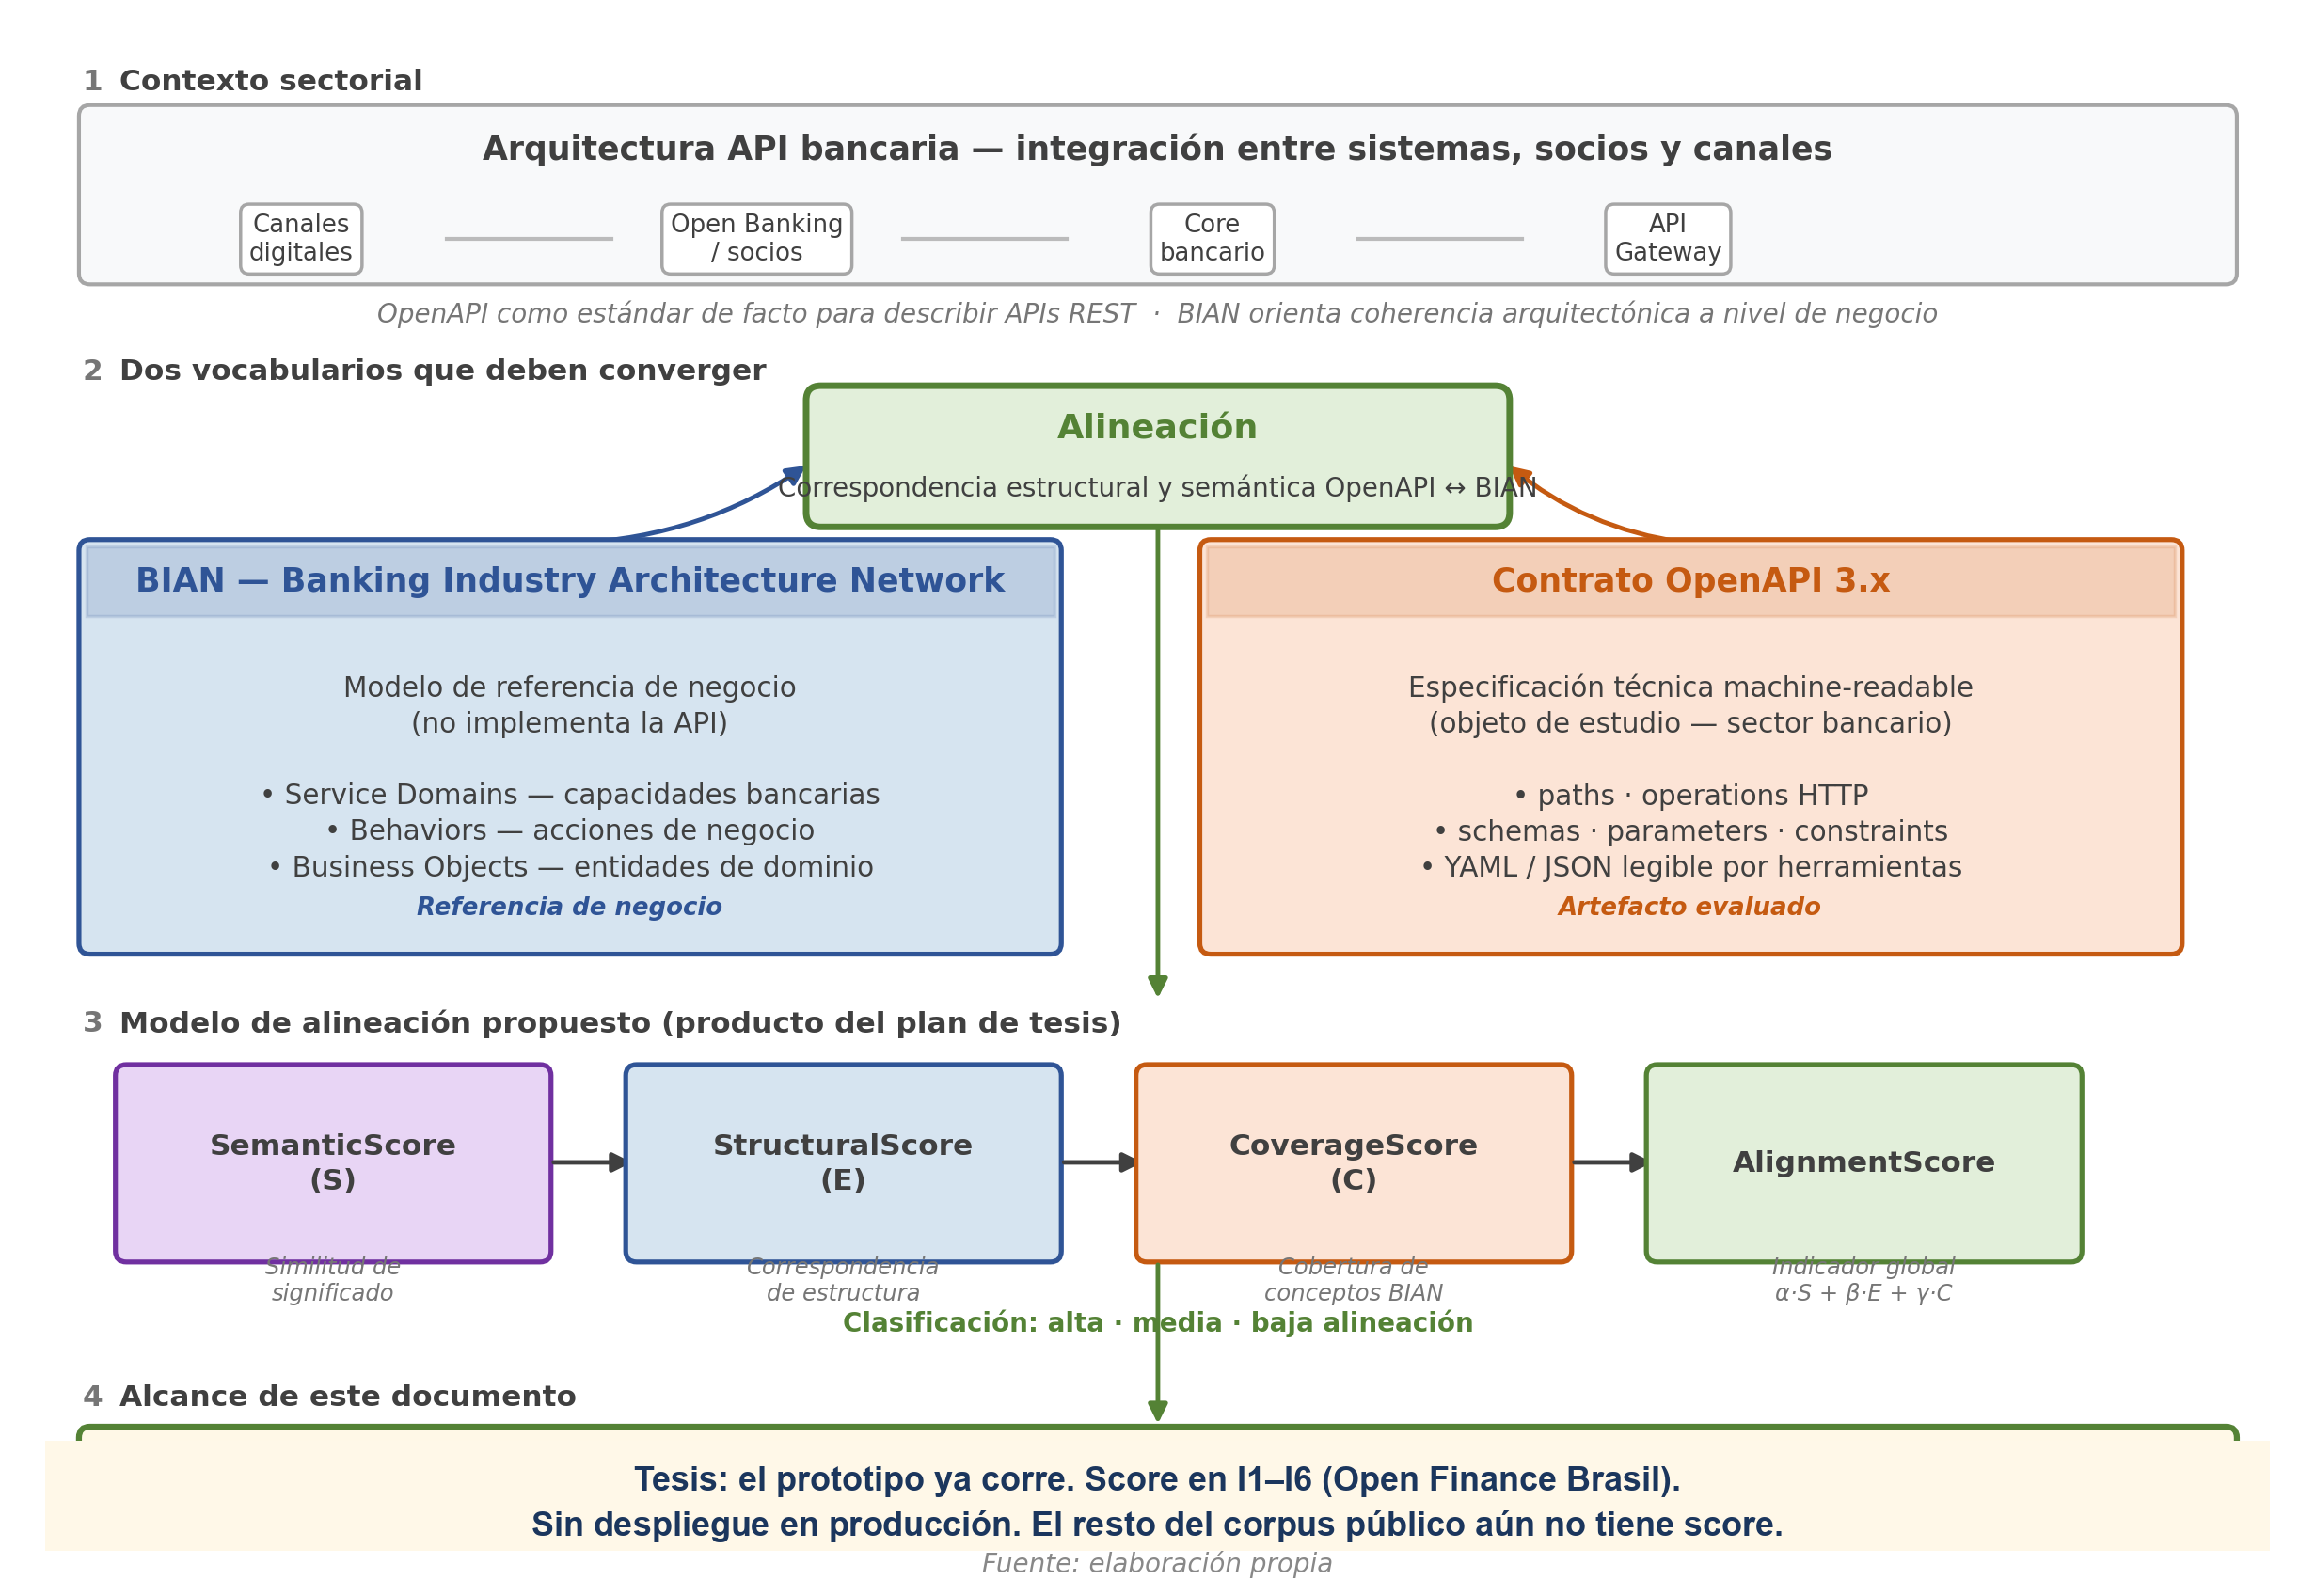
\includegraphics[width=0.92\textwidth]{Figura_01_Contexto}
  \caption{Contexto: arquitectura API bancaria, BIAN, OpenAPI y modelo S/E/C}
  \label{fig:contexto}
\end{figure}

\begin{figure}[H]
  \centering
  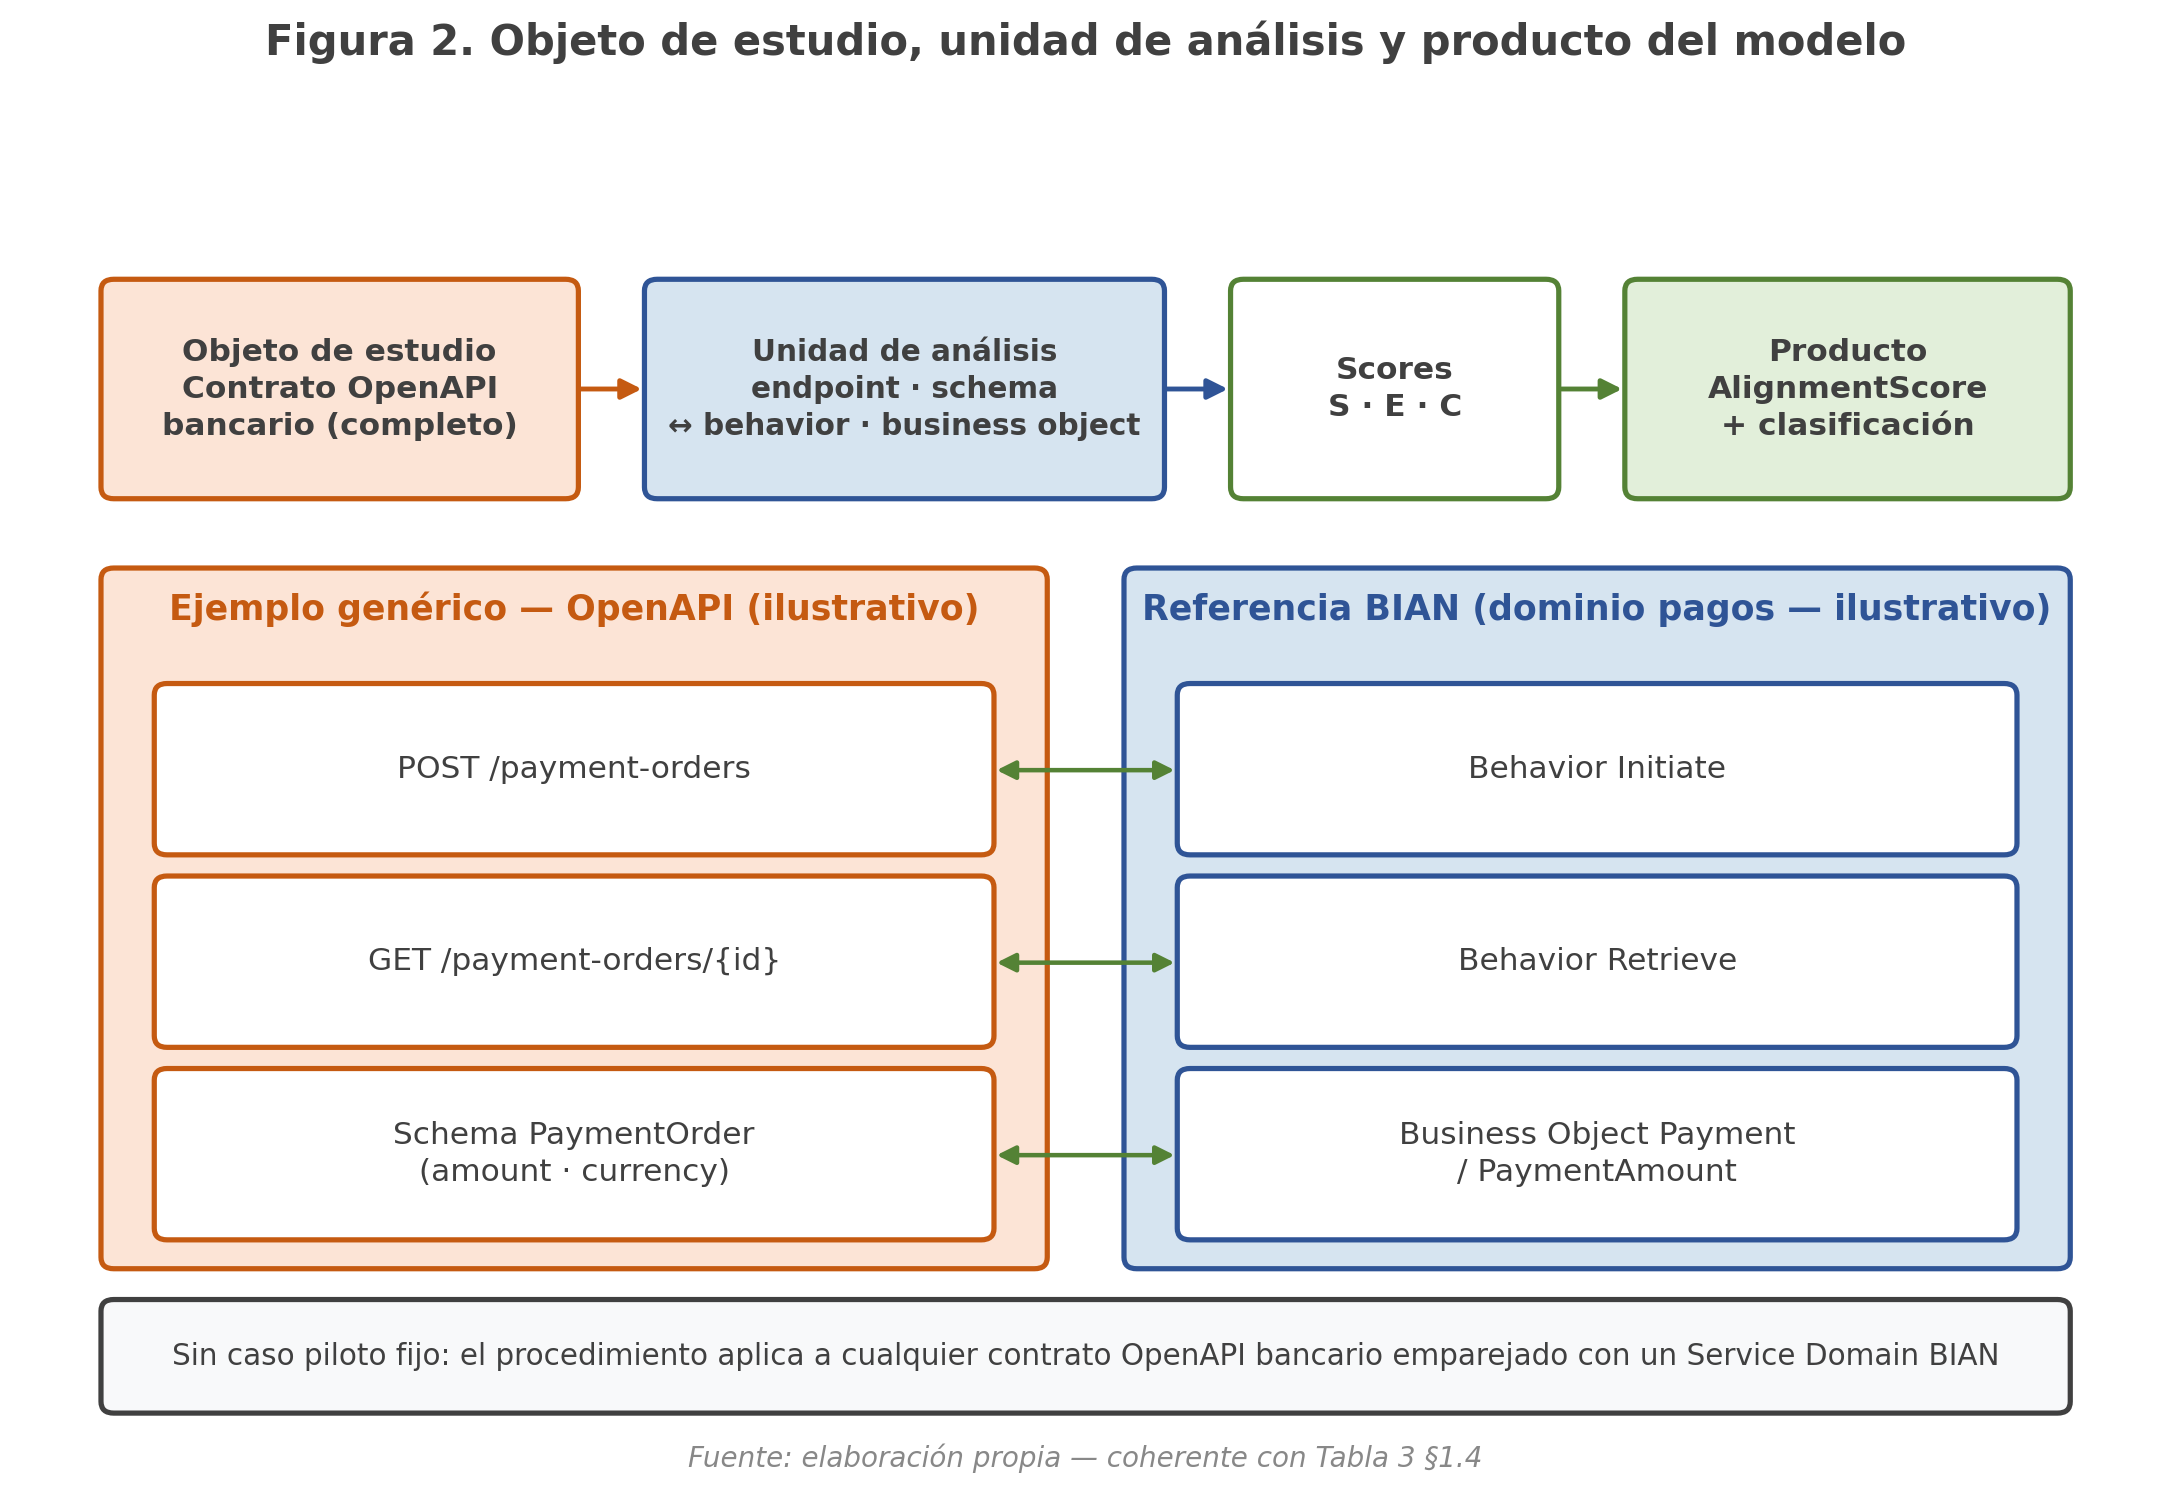
\includegraphics[width=0.88\textwidth]{Figura_02_Objeto_Unidad_Analisis}
  \caption{Objeto, referencia BIAN, unidad de análisis y producto del modelo}
  \label{fig:objeto}
\end{figure}

\begin{table}[H]
  \centering
  \caption{Objeto, unidad de análisis y producto}
  \label{tab:objeto}
  \begin{tabular}{@{}p{0.28\textwidth}p{0.62\textwidth}@{}}
    \toprule
    Concepto & En este estudio \\
    \midrule
    Objeto de estudio & El contrato OpenAPI bancario (el archivo) \\
    Unidad de análisis & Operación o esquema del contrato frente a un behavior o business object del Service Domain \\
    Producto & S, E, C y AlignmentScore por instancia contrato $\times$ dominio \\
    \bottomrule
  \end{tabular}
\end{table}

Cada instancia se nombra con la fuente, el dominio y la versión. I1 es \texttt{accounts} 2.4.2 contra Savings Account. El corpus público del capítulo III amplía las fuentes. No cambia el objeto.

\begin{table}[H]
  \centering
  \caption{Tipología de desalineaciones}
  \label{tab:tipologias}
  \small
  \begin{tabular}{@{}p{0.18\textwidth}p{0.38\textwidth}p{0.34\textwidth}@{}}
    \toprule
    Tipo & Qué es & Ejemplo \\
    \midrule
    Estructural & La organización de endpoints no sigue la del dominio & \texttt{POST /transfer} sin el behavior \texttt{Initiate} \\
    Semántica & La estructura se parece y el negocio no & \texttt{amount} sin vínculo con \texttt{PaymentAmount} \\
    De modelado & Falta una entidad o un atributo obligatorio & Un esquema que omite campos del business object \\
    REST / contrato & El verbo o la ruta no se leen como operación de negocio & Un verbo metido en la URL \\
    \bottomrule
  \end{tabular}
\end{table}

\section{Ámbito y delimitación}

El ámbito es el archivo público, no el banco. La tabla fija sector, artefactos, técnica, geografía y tiempo. Quedan fuera el despliegue, las pruebas de penetración y medir latencia en ejecución.

\begin{table}[H]
  \centering
  \caption{Ámbito del estudio}
  \label{tab:ambito}
  \begin{tabular}{@{}p{0.24\textwidth}p{0.66\textwidth}@{}}
    \toprule
    Dimensión & Delimitación \\
    \midrule
    Sector & Banca y servicios financieros con APIs \\
    Artefactos & Contratos OpenAPI o Swagger públicos, y Service Domains BIAN v14 \\
    Técnica & Análisis estructural y similitud semántica \\
    Geografía & No restringida. Los casos son documentación pública \\
    Tiempo & Especificaciones vigentes en 2024--2026. La lista de corpus se cerró el 21 de noviembre de 2026 \\
    \bottomrule
  \end{tabular}
\end{table}

\section{Alcances y limitaciones}
\label{sec:alcances}

El modelo ya está en un prototipo, y el piloto de siete instancias ya tiene número. La tabla separa eso de lo que sigue fuera: el YAML de un banco emisor, la corrida de todo el corpus contra los 258 dominios, y el despliegue. Los demás estándares públicos entran al corpus y, en este borrador, no tienen score.

\begin{table}[H]
  \centering
  \caption{Alcances y limitaciones}
  \label{tab:alcances}
  \footnotesize
  \begin{tabular}{@{}p{0.46\textwidth}p{0.46\textwidth}@{}}
    \toprule
    Alcance & Limitación \\
    \midrule
    Medir alineación estructural y semántica entre un contrato OpenAPI y un Service Domain & No desplegar APIs \\
    Dejar métricas que otra persona pueda repetir & No sustituir una certificación ni una auditoría legal \\
    El modelo S, E, C y el AlignmentScore & No puntuar los 258 dominios contra todo el corpus \\
    El corpus de contratos públicos del capítulo III & FDX y los PDF sin YAML no entran al parser \\
    El prototipo y el piloto de siete instancias, ya corrido & El resto del corpus todavía no tiene score \\
    Niveles Alta, Media, Baja y Nula & Los cortes son convención. No hay F1 \\
    \bottomrule
  \end{tabular}
\end{table}

\section{Justificación}

Si un release mueve el YAML y el Service Domain se queda en el modelo, el desfase se ve en el archivo: un path nuevo, un \texttt{operationId} que ya no nombra el behavior, un \texttt{\$ref} que apunta a otro esquema. Farzi \cite{Farzi2021} y Bhatia \cite{Bhatia2022} describen esa deriva entre producto, integración y gobernanza cuando el contrato y BIAN no se rastrean. Conviene verla en el archivo, no cuando el servicio ya está en producción.

Revisar a mano no escala cuando hay decenas de APIs y de socios. El AlignmentScore ordena esa cola con un número \cite{Shabbir2025}. OpenAPI, como artefacto, ya está maduro \cite{Casas2021}. Lo que no teníamos escrito es el cruce con un Service Domain. El procedimiento de esta tesis es esa pieza.

La pregunta cabe en el archivo. Este contrato, en esta versión, ¿refleja este Service Domain? S y E salen de ahí. No son una prueba en ejecución, ni un sello.

\section{Clasificación IEEE / ACM}

El tema cae en representación de conocimiento y en redes semánticas. No es testing de APIs ni un clasificador entrenado con nuestros pares.

\begin{table}[H]
  \centering
  \caption{Clasificación IEEE / ACM}
  \label{tab:clasificacion}
  \begin{tabular}{@{}p{0.16\textwidth}p{0.28\textwidth}p{0.46\textwidth}@{}}
    \toprule
    Taxonomía & Categoría & Por qué \\
    \midrule
    IEEE & Knowledge Representation &
    El contrato y el Service Domain son dos representaciones del mismo negocio. Medimos si se corresponden \\
    ACM & Semantic networks &
    El emparejamiento y la similitud entre conceptos de negocio y piezas de la API caen en redes de significado y en alineación de esquemas \\
    \bottomrule
  \end{tabular}
\end{table}

\section{Hipótesis de trabajo}

No las contrastamos en este borrador. Cada una nombra el producto de un objetivo y el ratio que se mediría cuando haya etiquetas.

\begin{enumerate}
  \item H1, ligada a OE1. Normalizar el contrato y el dominio en la misma tabla permite calcular S, E y C. El ratio es la completitud de la extracción.
  \item H2, ligada a OE2. El schema matching de Shvaiko y Euzenat \cite{Shvaiko2005} produce un StructuralScore de la correspondencia REST--dominio.
  \item H3, ligada a OE3. La similitud semántica \cite{ElBayadh2015,Chandrasekaran2022} produce un SemanticScore que separa un concepto alineado de uno que no lo está.
  \item H4, ligada a OE4. La media de S, E y C produce un AlignmentScore que se puede clasificar por nivel.
\end{enumerate}

\section{Factores y ratios}

Los factores son decisiones de diseño. Los ratios son los números. En esta corrida los factores ya están elegidos: tabla y no grafo, greedy con los pesos 0,40 / 0,25 / 0,20 / 0,15, S léxico y MiniLM, pesos iguales en el score oficial.

\begin{table}[H]
  \centering
  \caption{Factores y ratios}
  \label{tab:variables}
  \footnotesize
  \begin{tabular}{@{}p{0.12\textwidth}p{0.28\textwidth}p{0.24\textwidth}p{0.26\textwidth}@{}}
    \toprule
    Pieza & Factor & Ratio & Control \\
    \midrule
    OG & Pesos del AlignmentScore & Score y nivel & $\alpha+\beta+\gamma=1$. Cortes fijos \\
    OE1 & Representación intermedia & Extraídos / esperados & Versión fija del YAML y del dominio \\
    OE2 & Regla de matching & E en $[0,1]$ & Mismos pares normalizados \\
    OE3 & Encoder & S en $[0,1]$ & Mismos pares. Sin fine-tuning \\
    OE4 & Pesos & C, y el score global & Los tres pesos suman 1 \\
    \bottomrule
  \end{tabular}
\end{table}

\begin{figure}[H]
  \centering
  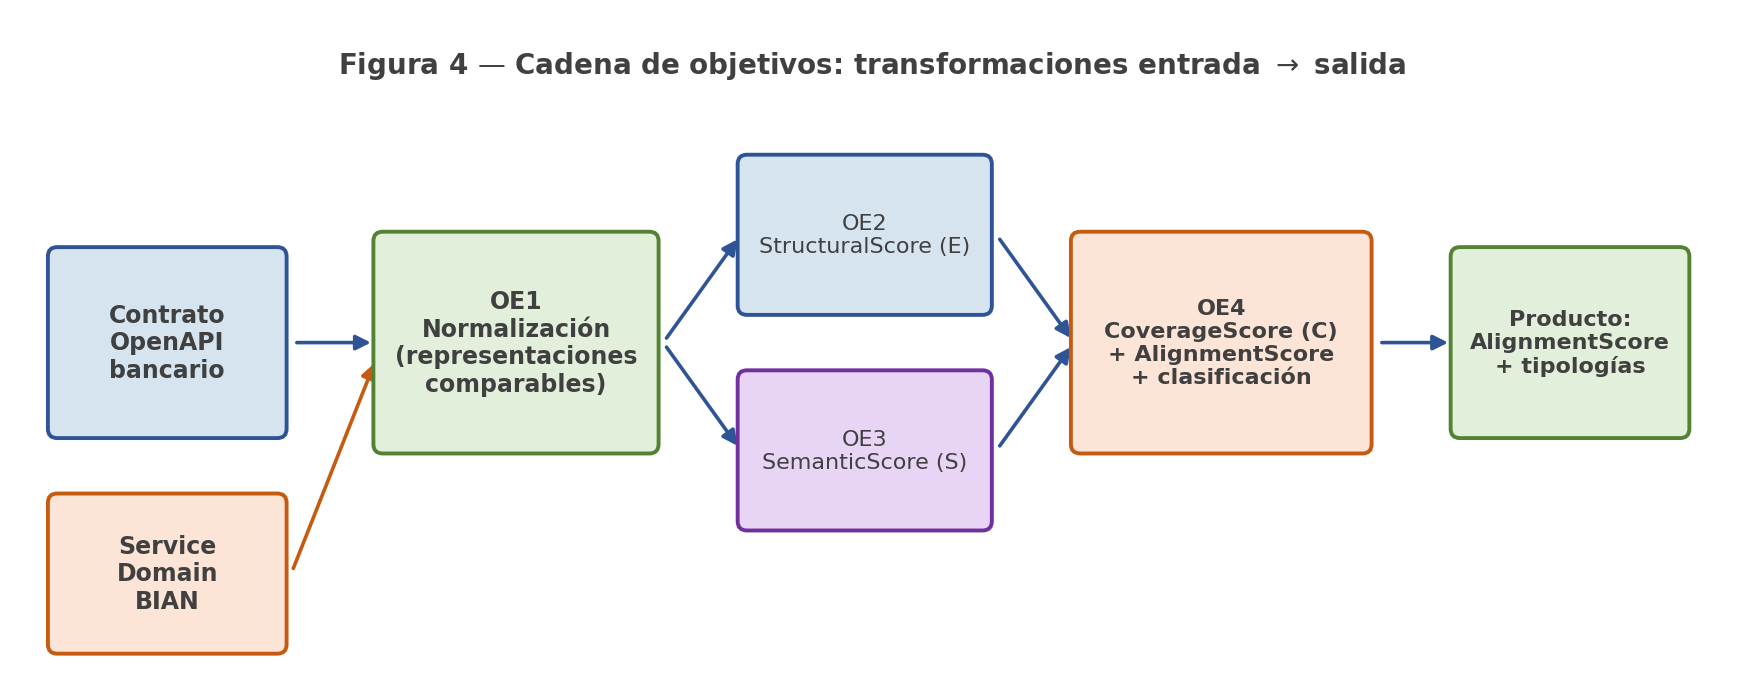
\includegraphics[width=0.98\textwidth]{Figura_04_Cadena_Objetivos}
  \caption{Cadena: normalizar, calcular S, E y C, integrar el AlignmentScore}
  \label{fig:cadena}
\end{figure}


\chapter{Marco teórico}

\section{Antecedentes bibliográficos}

Partimos el corpus en seis ejes. No todos pesan lo mismo para el score. La tabla junta el hallazgo, qué pieza del score toca, y el hueco que nos queda.

\begin{table}[H]
  \centering
  \caption{Síntesis de los seis ejes}
  \label{tab:ejes}
  \footnotesize
  \begin{tabular}{@{}p{0.08\textwidth}p{0.28\textwidth}p{0.22\textwidth}p{0.28\textwidth}@{}}
    \toprule
    Eje & Papers & Aporte & Hueco \\
    \midrule
    E1 & Casas; Mainas; Santos y Casas & El contrato como artefacto. Mainas alimenta S & Sin Service Domain \\
    E2 & Shvaiko y Euzenat & La taxonomía de E & Sin REST ni banca \\
    E3 & El Bayadh; Chandrasekaran; Santos Sousa; He; Schneider; Hertling & S por similitud. C solo de paso & Sin OpenAPI bancario \\
    E4 & Schmidt; Lu; Kotstein; Oberle & Dominio hacia interfaz & El segundo archivo sigue siendo una API \\
    E5 & Ehsan; Golmohammadi; Otieno; Tanveer; Vitorino & Queda fuera. Es testing & No es el AlignmentScore \\
    E6 & Mahanra Rao & S parcial, por ranking & Elegir un servicio no es alinearlo con BIAN \\
    \bottomrule
  \end{tabular}
\end{table}

\subsection{OpenAPI como contrato}

Casas et al.\ \cite{Casas2021} revisan 47 artículos de 2011 a 2020. OpenAPI queda como la descripción REST que una máquina puede leer. El uso que encuentran es generar código, probar y gobernar. El 68\,\% propone herramientas y el 43\,\% mejora la documentación. En esos 47 el contrato no queda al lado de un Service Domain. Mainas et al.\ \cite{Mainas2023} anotan el contrato (\texttt{x-refersTo}, \texttt{x-kindOf}, \texttt{x-mapsTo}), lo pasan a RDF y consultan con SPARQL más de 300 especificaciones de SwaggerHub. Un YAML de más de 200 líneas les llevó más de un segundo. No definen un SemanticScore, y el corpus es SwaggerHub, no banca. Santos y Casas \cite{SantosCasas2025}, con \textit{design science}, catalogan 59 métricas de API Gateway (latencia, tráfico, errores) en 68 productos. Eso es calidad en producción. No es el cruce del YAML con un Service Domain.

\subsection{Emparejamiento de esquemas}

Shvaiko y Euzenat \cite{Shvaiko2005} ordenan el \textit{schema matching} en tres cortes: exacto o aproximado; evidencia sintáctica, semántica o externa; elemento o estructura. El trabajo es anterior a OpenAPI y a JSON Schema. El StructuralScore usa el corte aproximado. La evidencia es el nombre, la ruta y el verbo. El grano es la operación, no el archivo entero. \textit{Paths}, operaciones y \textit{schemas} se leen contra behaviors y business objects. No traen un corpus bancario. La métrica que se puede repetir sobre ese par la fijamos nosotros, en el capítulo III.

\subsection{Similitud y ontologías}

El Bayadh et al.\ \cite{ElBayadh2015} separan la alineación ontológica en terminológica, estructural, extensional y semántica. Avistan que una sola medida no basta y que una combinación fija puede quedar corta. Por eso S, E y C no se sustituyen entre sí, y los pesos iguales del AlignmentScore se acompañan de dos juegos de sensibilidad. Chandrasekaran y Mago \cite{Chandrasekaran2022} recorren la similitud desde WordNet hasta los \textit{transformers}. Santos Sousa et al.\ \cite{SantosSousa2026} listan tres límites de los \textit{embeddings} en ontology matching: hace falta supervisión, la escala pesa, y hay correspondencias que no son uno a uno.

Tres trabajos recientes dicen qué encoder usar y qué no ajustar. He et al.\ \cite{He2022} fine-tunean BERT (BERTMap) sobre el texto de la ontología y reparan el alineamiento con la estructura. Schneider et al.\ \cite{Schneider2023} codifican la etiqueta con un \textit{sentence transformer} ya entrenado y comparan por coseno, sin ajuste. Hertling y Paulheim \cite{Hertling2023} le preguntan a un modelo grande, con pocos ejemplos, si dos entidades coinciden. Nos quedamos con el coseno de Schneider et al. No copiamos el ajuste de He et al.: no hay una ontología BIAN etiquetada. El par no lo arma un chat.

\subsection{Dominio e interfaz}

Schmidt y Thiry \cite{Schmidt2020} revisan 27 estudios primarios, de 715 registros entre 2013 y 2019, sobre cómo identificar microservicios con MDE y DDD. Un Service Domain puede ser la referencia de negocio y la API la capa que lo expone. Esa revisión no calcula un desfase. Lu et al.\ \cite{Lu2024} agrupan microservicios parecidos con GloVe sobre el OpenAPI entero. Kotstein y Decker \cite{Kotstein2024} ajustan BERT con 2\,321 especificaciones para señalar un endpoint a partir de una pregunta. Oberle y Bauernhansl \cite{Oberle2024} comparan TF-IDF, word2vec, fastText y embeddings sobre 326 endpoints de un MES, con corte de expertos. En los tres el segundo archivo también es una API. Nosotros ponemos al lado un Service Domain.

\subsection{Lo que no entra}

Ehsan et al.\ \cite{Ehsan2022} cubren 16 artículos de testing RESTful. La métrica que domina es el \textit{code coverage}. Golmohammadi et al.\ \cite{Golmohammadi2024} leen 92 papers que generan casos sobre endpoints ya vivos. Otieno y Araka \cite{Otieno2026} ponen aprendizaje automático en las pruebas y se quejan de datasets chicos. Tanveer et al.\ \cite{Tanveer2025} van a vulnerabilidades. Vitorino et al.\ \cite{Vitorino2025}, a datos adversariales. Aquí OpenAPI es la entrada de una prueba. En esta tesis es el artefacto que se contrasta con el dominio. Mahanra Rao et al.\ \cite{MahanraRao2025} revisan 25 estudios (2020--2024) que usan BERT para elegir un servicio según su QoS. El ranking no es el AlignmentScore.

\section{Bases teóricas}

El StructuralScore se apoya en Shvaiko y Euzenat \cite{Shvaiko2005}: correspondencia entre esquemas, no un clasificador. El aviso de El Bayadh et al.\ \cite{ElBayadh2015} justifica no fiar el expediente a una sola medida. El SemanticScore de esta corrida es el coseno de un encoder de frases ya entrenado \cite{Schneider2023,Reimers2019}, no un BERT ajustado a BIAN \cite{He2022} ni una pregunta a un modelo generativo \cite{Hertling2023}.

El Bayadh separa cuatro familias. La terminológica es el S léxico, y en el piloto se queda entre 0,00 y 0,03: el YAML está en portugués y el dominio en inglés. La estructural es E. La semántica es el coseno de MiniLM. La extensional pediría filas de datos, movimientos, saldos reales. El archivo no las trae. Trae el contrato.

Mainas et al.\ \cite{Mainas2023} pasan el YAML a RDF, con una ontología REST. OE1 no hace eso. Deja una fila por operación. El vocabulario del score sale de esa tabla y del dominio ya normalizado. No sale de un texto suelto.

Dado un contrato y un Service Domain emparejado, el procedimiento normaliza, calcula S, E y C, y junta

\[
\mathrm{AlignmentScore} = \alpha S + \beta E + \gamma C, \qquad \alpha+\beta+\gamma = 1.
\]

En la corrida oficial $\alpha = \beta = \gamma = 1/3$. La sensibilidad usa $(0{,}50,\ 0{,}30,\ 0{,}20)$ y $(0{,}20,\ 0{,}50,\ 0{,}30)$ sin cambiar el número oficial. El nivel es Alta si el score llega a 0,80, Media entre 0,60 y 0,79, Baja entre 0,40 y 0,59, y Nula por debajo de 0,40. Esos cortes no se aprenden.

CoverageScore no es el \textit{code coverage} de las pruebas \cite{Ehsan2022}. Es la fracción de tags \texttt{CR} y \texttt{BQ} del Service Domain que recibieron al menos un par. S se promedia solo sobre los pares que el greedy dejó. Las operaciones del contrato que se quedaron solas entran en E como cero, y no entran en S.

\section{Definición de términos}

Abajo, el vocabulario del score. Alineación es el cruce entre el archivo y el dominio. No nombra al banco.

\begin{table}[H]
  \centering
  \caption{Términos que usa el modelo}
  \label{tab:terminos}
  \small
  \begin{tabular}{@{}p{0.28\textwidth}p{0.64\textwidth}@{}}
    \toprule
    Término & Qué significa aquí \\
    \midrule
    Contrato OpenAPI & YAML o JSON (OpenAPI 3.x, o Swagger 2 cuando el estándar no migró) con \textit{paths}, operaciones y \textit{schemas}. \\
    Service Domain & Unidad de negocio BIAN: behaviors, business objects y relaciones de control. \\
    Behavior & Acción de negocio definida en el Service Domain. \\
    Business object & Entidad del dominio (una orden de pago, una cuenta) referida en el modelo. \\
    SemanticScore (S) & Parecido de significado entre los textos emparejados, en $[0,1]$. \\
    StructuralScore (E) & Correspondencia de nombre, ruta, verbo y profundidad, en $[0,1]$. No es una métrica de \textit{runtime}. \\
    CoverageScore (C) & Fracción de tags \texttt{CR}/\texttt{BQ} del dominio que recibieron par, en $[0,1]$. \\
    AlignmentScore & $(S+E+C)/3$ en la corrida oficial, con nivel Alta, Media, Baja o Nula. \\
    Schema matching & Correspondencia entre esquemas. Base de E \cite{Shvaiko2005}. \\
    Alineación & Correspondencia estructural y semántica entre el contrato y un Service Domain. \\
    Desalineación & Una de las cuatro de la tipología del capítulo I: estructural, semántica, de modelado, o de verbo y ruta. \\
    Instancia & Un contrato ya elegido contra un Service Domain ya elegido. I1 es \texttt{accounts} 2.4.2 contra Savings Account. No es el producto de los 38 YAML por los 258 dominios. \\
    Tag CR / BQ & Etiqueta del YAML de BIAN. CR es el registro de control del dominio. BQ califica un behavior, como Charge o Deposit. C es la fracción de esos tags que recibió al menos un par. \\
    Nivel & Alta, Media, Baja o Nula, con cortes fijos. No es una clase aprendida. \\
    \bottomrule
  \end{tabular}
\end{table}

\section{Brecha}

Los veinte papers del Anexo~\ref{anexo:papers}, leídos en cruz, dejan cinco cosas distintas. Casas et al.\ \cite{Casas2021} muestran el formato en 47 artículos, y Mainas et al.\ \cite{Mainas2023} prueban que el YAML se puede anotar. Shvaiko y Euzenat \cite{Shvaiko2005} dejan la taxonomía para cruzar esquemas. El Bayadh et al.\ \cite{ElBayadh2015} avisan que una medida no basta, y Santos Sousa et al.\ \cite{SantosSousa2026} dicen dónde fallan los embeddings: supervisión, escala, y pares que no son uno a uno. Schmidt y Thiry \cite{Schmidt2020} separan el dominio de la interfaz. BIAN puede ocupar ese lugar de referencia. Ehsan et al.\ \cite{Ehsan2022} y Golmohammadi et al.\ \cite{Golmohammadi2024} usan el contrato para probar APIs vivas. Mahanra Rao et al.\ \cite{MahanraRao2025} rankean servicios por calidad de servicio.

Casas y Mainas se quedan en el contrato. Shvaiko y El Bayadh no traen un YAML de banco. Schmidt separa el dominio de la interfaz y no calcula el desfase. Nosotros ponemos el Service Domain al lado del archivo y guardamos el AlignmentScore, para que otro pueda repetir el número.

\begin{table}[ht]
  \centering
  \caption{Vacíos V1 a V5}
  \label{tab:vacios}
  \footnotesize
  \begin{tabular}{@{}p{0.22\textwidth}p{0.34\textwidth}p{0.34\textwidth}@{}}
    \toprule
    Vacío & De dónde sale & Qué hacemos con eso \\
    \midrule
    V1. OpenAPI y BIAN juntos & El review no estudia los dos artefactos en banca & El objeto sigue siendo el contrato. BIAN es la referencia, y ese cruce no está en el review \\
    V2. Una métrica sola no alcanza & E2 y E3 aportan técnicas sueltas & S, E, C y el AlignmentScore \\
    V3. Cobertura & El matching ontológico habla de cobertura, no de business objects BIAN dentro del YAML & CoverageScore \\
    V4. Un procedimiento que se repita & Mainas et al.\ arman RDF. No dejan un score ni un nivel & El prototipo del capítulo III \\
    V5. Antes del despliegue & E5 y E6 miran runtime o ranking & El score es documental \\
    \bottomrule
  \end{tabular}
\end{table}

\begin{figure}[ht]
  \centering
  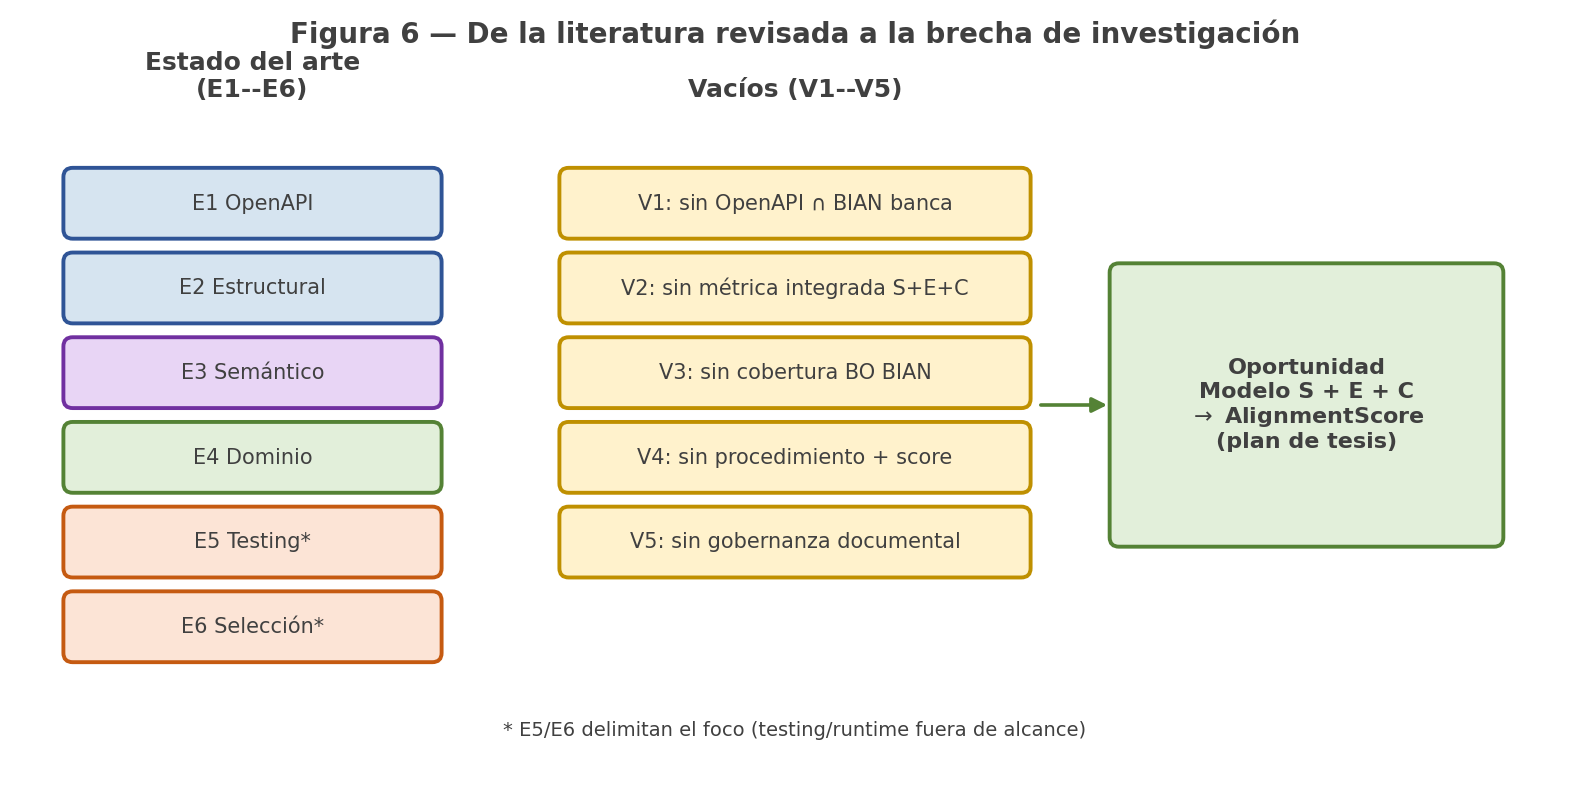
\includegraphics[width=0.92\textwidth]{Figura_06_Brecha}
  \caption{De los ejes E1--E6 a los vacíos V1--V5}
  \label{fig:brecha}
\end{figure}

\begin{figure}[ht]
  \centering
  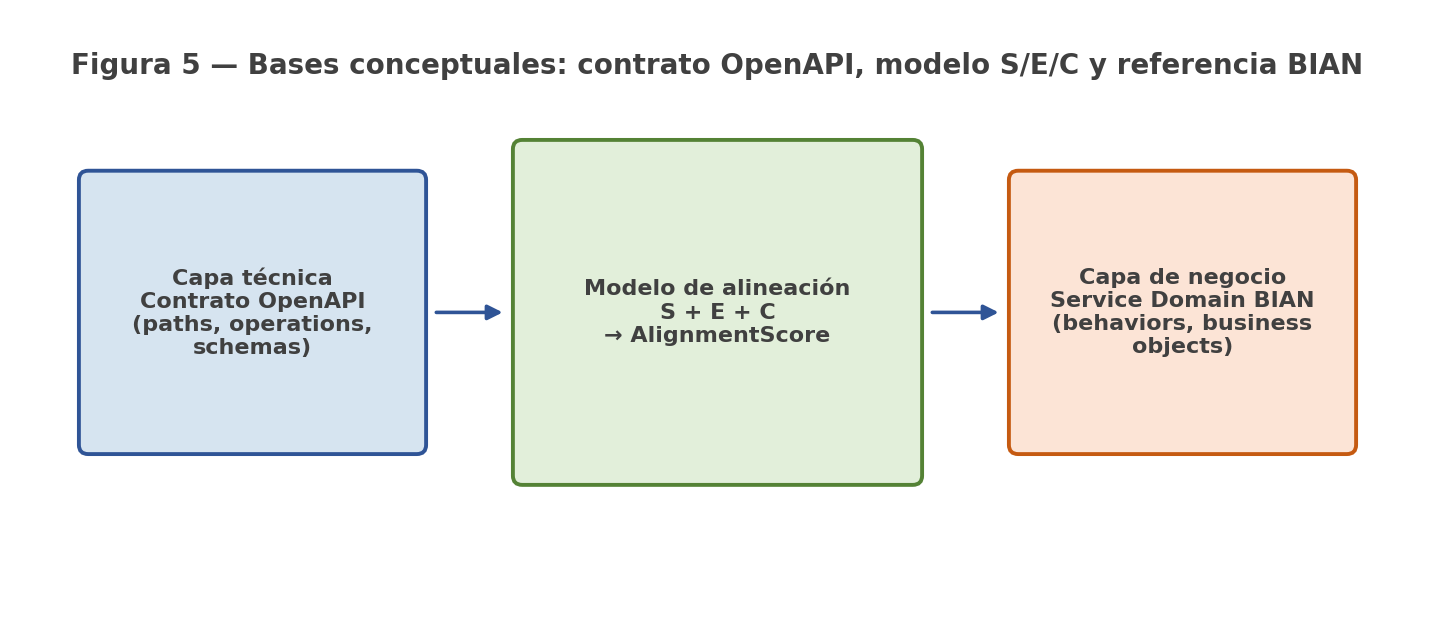
\includegraphics[width=0.88\textwidth]{Figura_05_Bases_Conceptuales}
  \caption{Contrato OpenAPI, Service Domain y modelo S/E/C}
  \label{fig:bases}
\end{figure}

He et al.\ \cite{He2022}, Schneider et al.\ \cite{Schneider2023} y Hertling y Paulheim \cite{Hertling2023} están en E3. Lu et al.\ \cite{Lu2024}, Kotstein y Decker \cite{Kotstein2024} y Oberle y Bauernhansl \cite{Oberle2024} están en E4. Entran como técnica del encoder y del parecido entre APIs. No arman el par contrato--Service Domain.


\chapter{Propuesta y desarrollo de la solución}

Los números de este capítulo salen de la corrida del 6 de noviembre de 2026. Quedó firmada en \texttt{results/matching/oe1\_firma.json} (fecha \texttt{2026-11-06T21:00:02Z}). El código que hoy permite repetirla está en \url{https://github.com/denniskano/piloto-bank-api-bian}, commit \texttt{12c1c04}. No recalculamos los scores el 21 de noviembre.

\section{Presentación de la propuesta de solución}

El objetivo general pide un número por par contrato $\times$ dominio. La propuesta es un prototipo con cuatro programas. Cada uno lee la salida del anterior.

\begin{enumerate}
  \item \path{python -m ofb_bian.procesar_openapi} lee los YAML y escribe \path{results/consolidado/}. Esos CSV no van a GitHub. Se regeneran.
  \item \texttt{python -m ofb\_bian.matching\_v0} arma los pares de I1 a I6 y calcula E, el S léxico y C.
  \item \texttt{python -m ofb\_bian.matching\_s1} recalcula solo S, con MiniLM, sobre los pares que congeló el paso anterior. E y C no se tocan.
  \item \texttt{python -m ofb\_bian.mapa\_ofb\_bian} es un catálogo extra (préstamos, tarjetas, inversiones). No entra en $n = 7$.
\end{enumerate}

No corrimos las 38 APIs contra los 258 dominios. No hay YAML de un banco emisor. No entrenamos un clasificador.

\begin{table}[ht]
  \centering
  \caption{Qué quedó hecho el 6 de noviembre de 2026, por objetivo}
  \label{tab:oe}
  \small
  \begin{tabular}{@{}p{0.22\textwidth}p{0.40\textwidth}p{0.28\textwidth}@{}}
    \toprule
    Objetivo & Hecho & Falta \\
    \midrule
    OE1. Normalizar & Parser sobre 296 YAML. Firma 296/296. & El parser no aplana \texttt{allOf}. \\
    OE2. Estructural & Greedy uno a uno en I1--I6. Pares congelados. & Etiquetas de un lector. \\
    OE3. Semántico & S léxico y S MiniLM sobre esos pares. & No hay etiquetas para un ajuste. No lo hacemos. \\
    OE4. Integrar & AlignmentScore $= (S+E+C)/3$ y el nivel. & Precision, recall, F1 y kappa. \\
    \bottomrule
  \end{tabular}
\end{table}

\begin{figure}[ht]
  \centering
  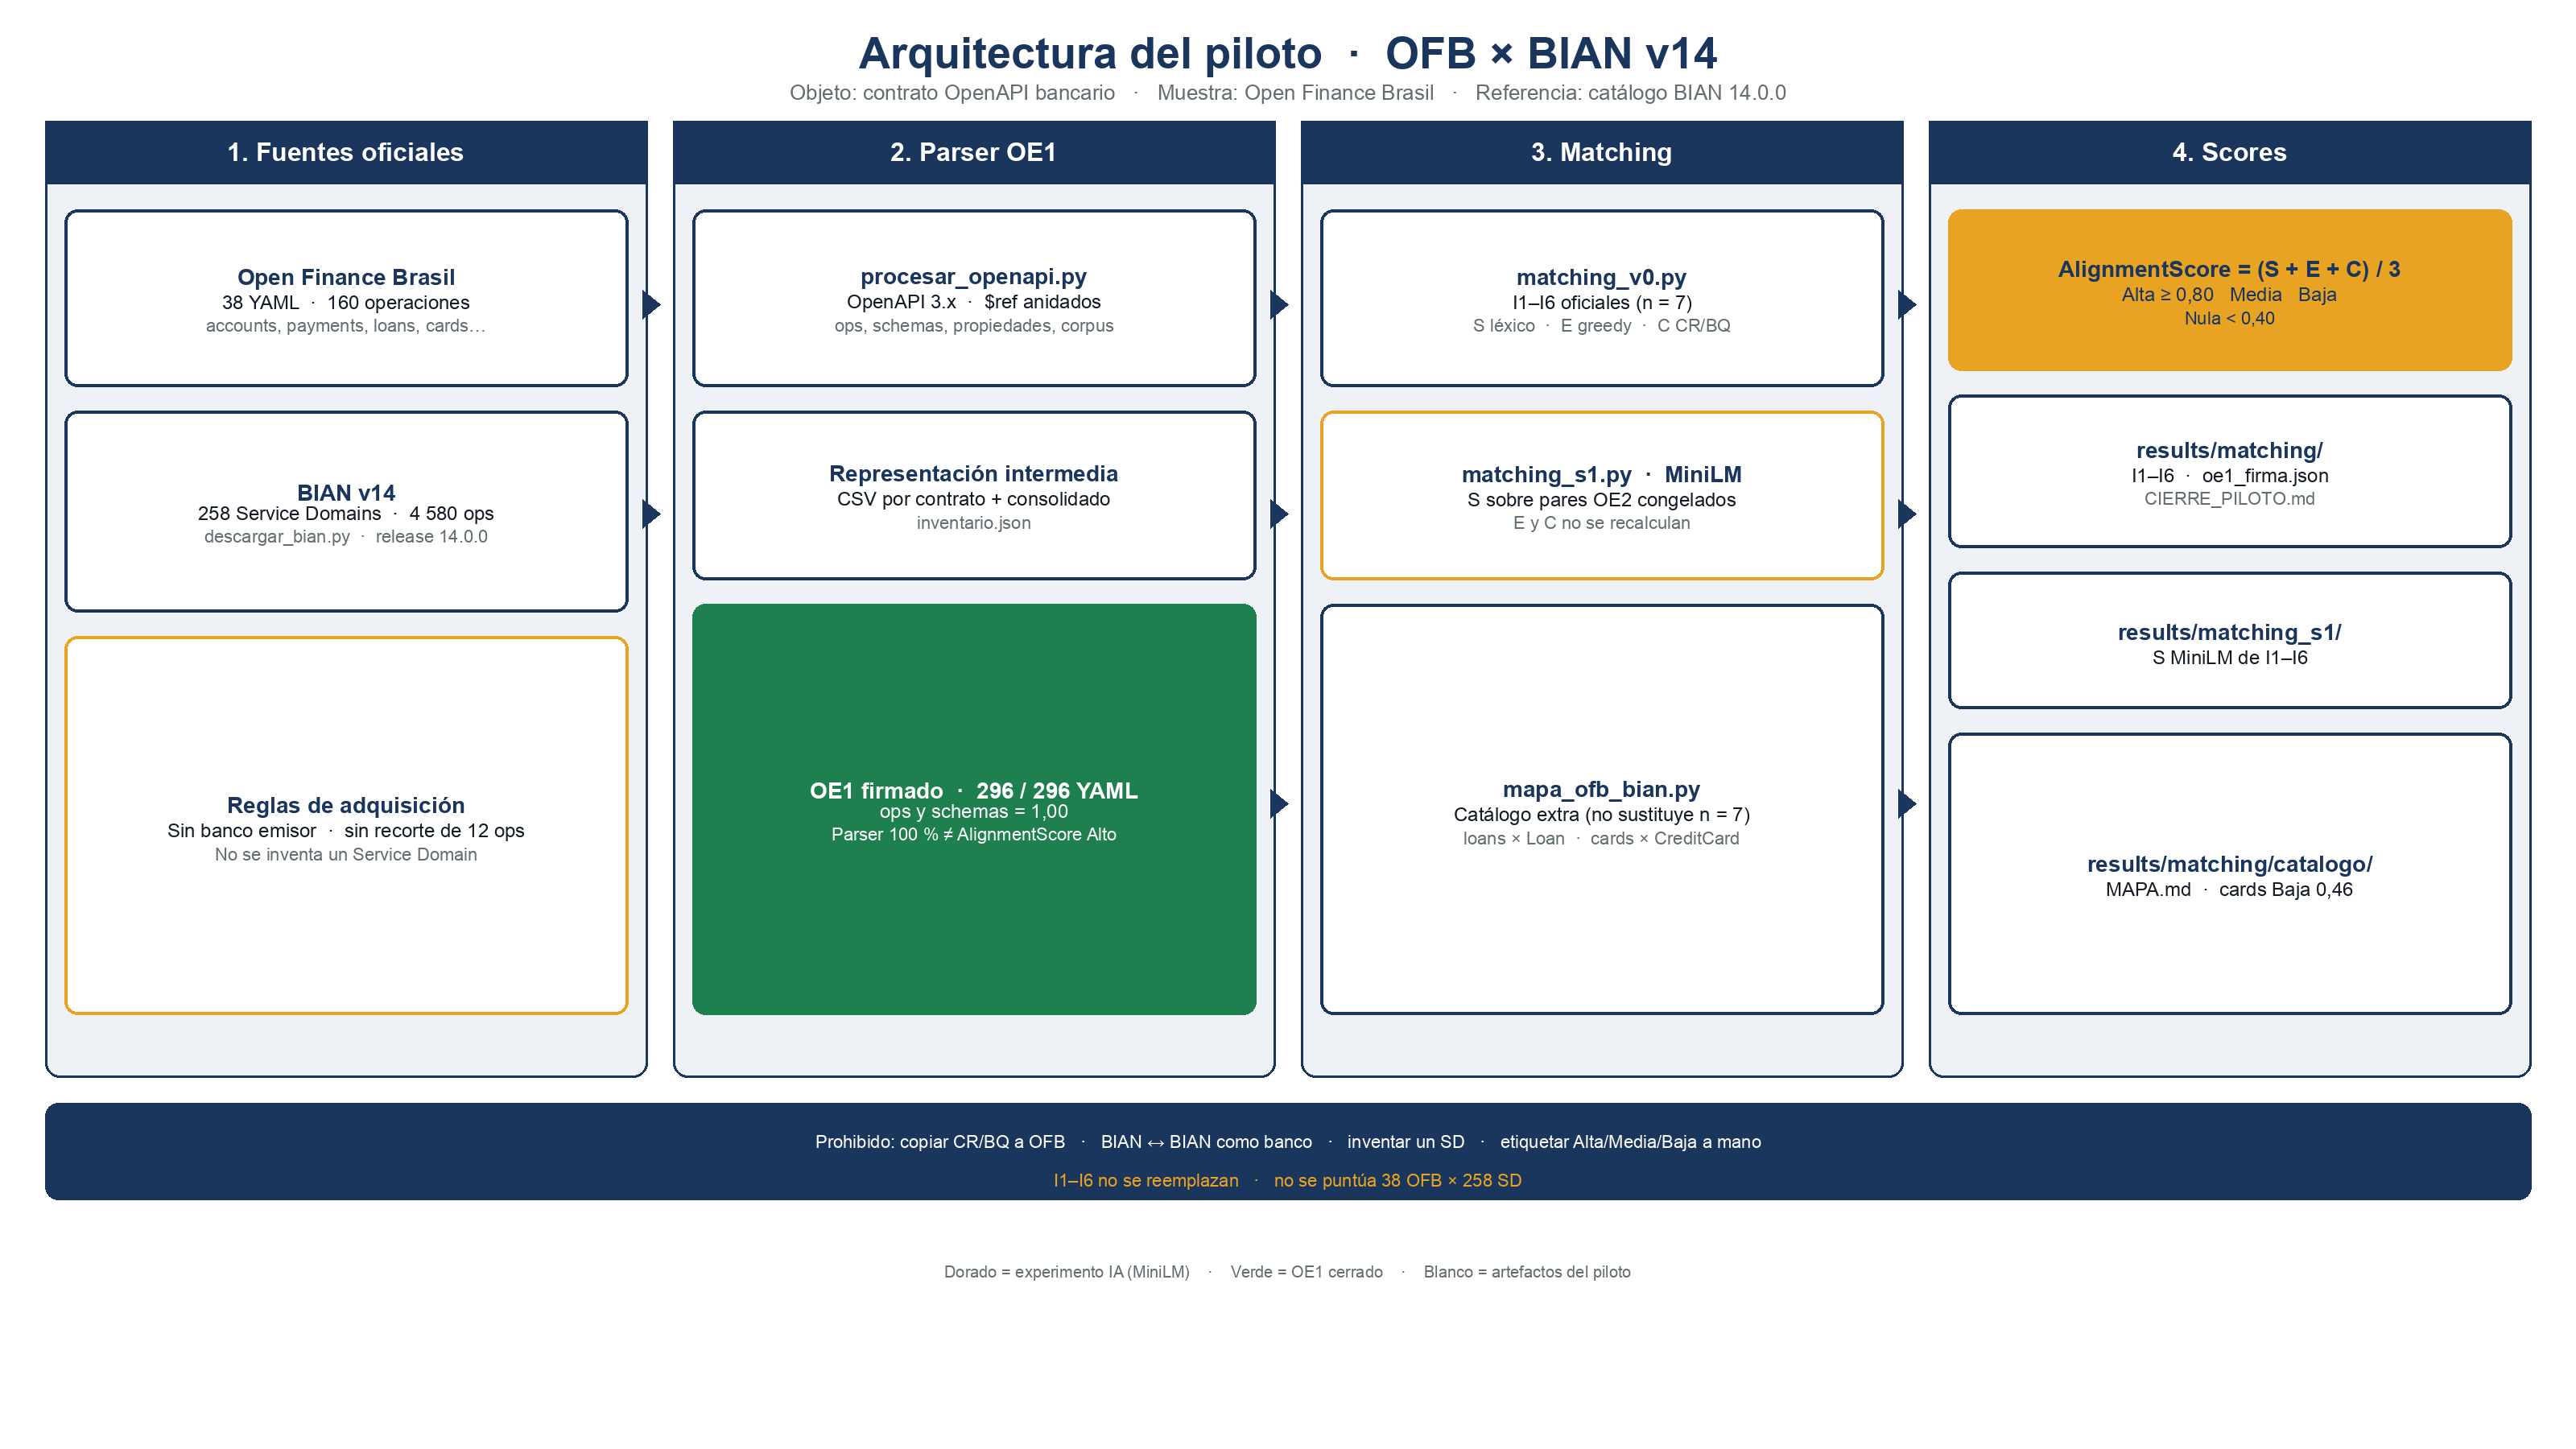
\includegraphics[width=\textwidth]{arquitectura-piloto}
  \caption{Pipeline que ya corrió sobre Open Finance Brasil. El corpus de la tesis es más ancho. Esos YAML todavía no pasan por estas cajas}
  \label{fig:arquitectura}
\end{figure}

\section{Desarrollo de la propuesta de solución}

\subsection{Datos}

La población sigue siendo cualquier par contrato OpenAPI bancario $\times$ Service Domain BIAN. El corpus de esta tesis son los contratos que el 21 de noviembre de 2026 se podían bajar sin cuenta. La referencia, en todos los casos, es BIAN v14.0.0 (258 Service Domains, 4\,580 operaciones, en \texttt{bian-official/public}). No hay datos personales. El parser lee OpenAPI 3.x y, si el estándar no migró, Swagger 2.

\begin{table}[ht]
  \centering
  \caption{Corpus de contratos públicos. Solo Open Finance Brasil tiene score en este borrador}
  \label{tab:corpus}
  \footnotesize
  \begin{tabular}{@{}p{0.22\textwidth}p{0.40\textwidth}p{0.14\textwidth}p{0.14\textwidth}@{}}
    \toprule
    Origen & Contrato & Idioma & En este borrador \\
    \midrule
    Brasil & Open Finance Brasil, 38 YAML & Portugués & Parseado. Score en I1--I6 \\
    Reino Unido & Read/Write v4.0.1 & Inglés & En el corpus. Sin score \\
    Europa & Berlin Group XS2A v1.3.16 & Inglés & En el corpus. Sin score \\
    Europa & Berlin Group openFinance, AIS 2.4.1 & Inglés & En el corpus. Sin score \\
    Francia & STET PSD2 1.6.3.2 & Inglés & En el corpus. Sin score \\
    Polonia & PolishAPI 3.0 & Polaco e inglés & En el corpus. Sin score \\
    Chequia & COBS 9.0.0 & Inglés & En el corpus. Sin score \\
    Australia & CDR banca 1.36.0 & Inglés & En el corpus. Sin score. Energía y telecomunicaciones no entran \\
    Nueva Zelanda & Payments NZ, cuentas v3.0.3 y pagos & Inglés & En el corpus. La licencia del README no está cerrada \\
    Baréin & CBB Open Banking v1.0.0 & Inglés & En el corpus. El YAML dice \texttt{TBC-licence} \\
    Emiratos & Open Finance, YAML en Nebras, pagos v2.1-errata3 & Inglés & En el corpus. El sitio se declara comunitario, no el repositorio de CBUAE \\
    \bottomrule
  \end{tabular}
\end{table}

\begin{figure}[ht]
  \centering
  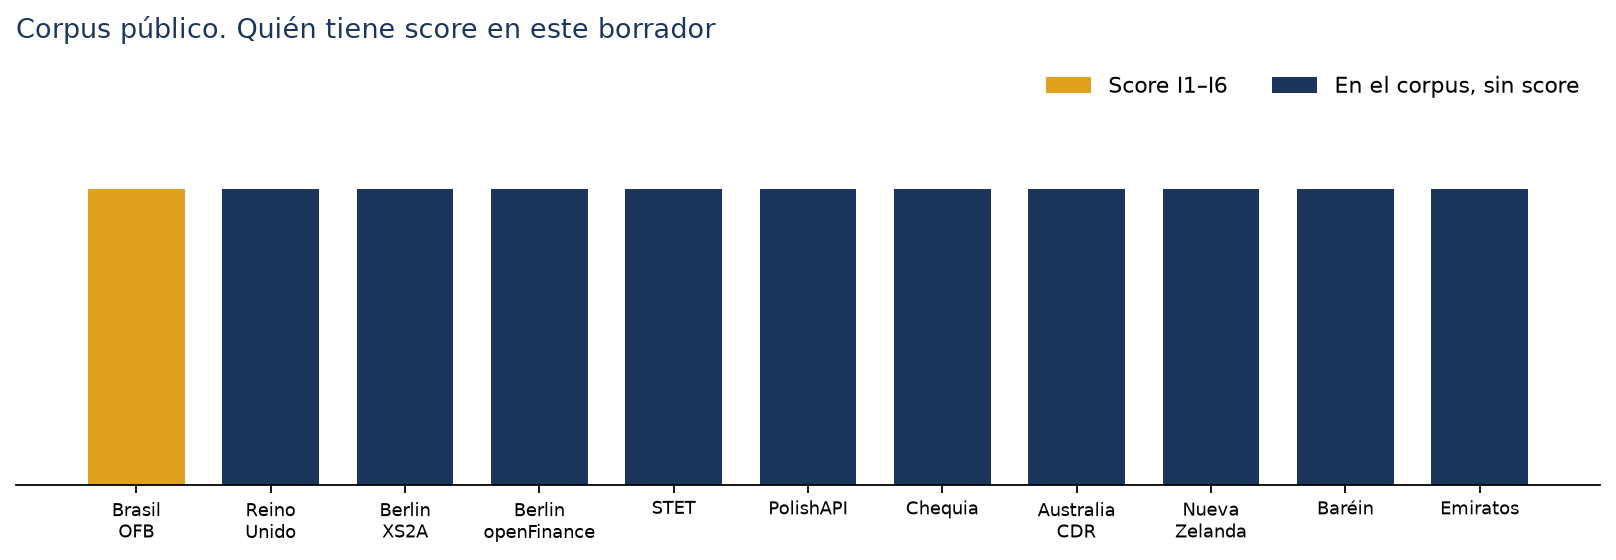
\includegraphics[width=\textwidth]{grafico-corpus}
  \caption{Once contratos públicos. Solo Open Finance Brasil tiene score en este borrador}
  \label{fig:corpus}
\end{figure}

\begin{figure}[ht]
  \centering
  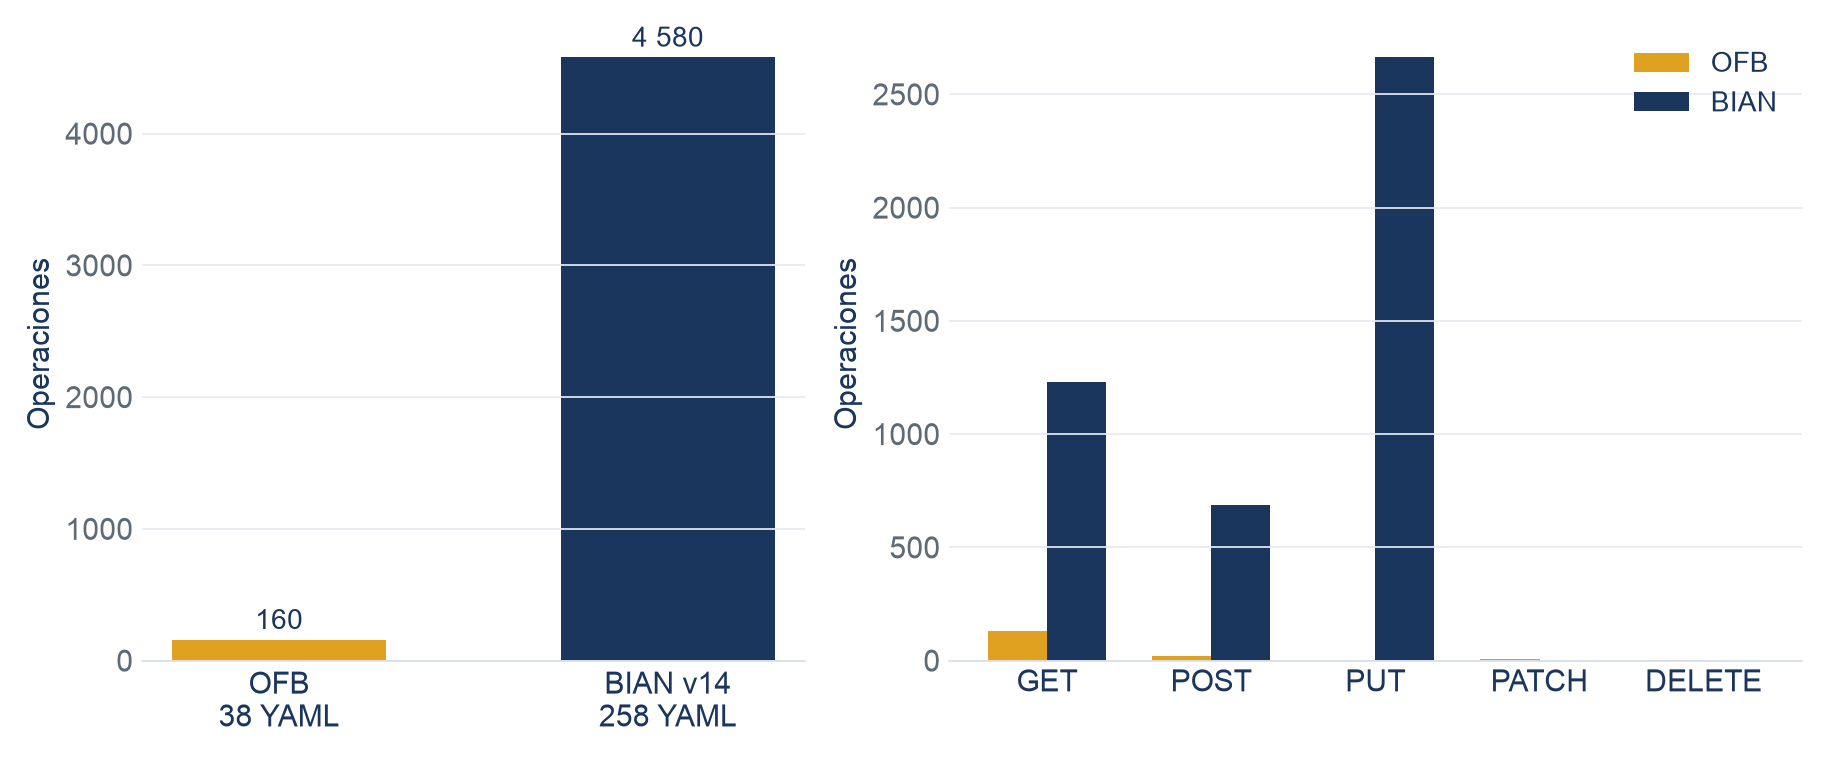
\includegraphics[width=0.92\textwidth]{grafico-fuentes}
  \caption{Operaciones del piloto ya parseado: 160 en OFB y 4\,580 en BIAN v14. OFB es sobre todo GET. BIAN es sobre todo PUT}
  \label{fig:fuentes}
\end{figure}

Tres archivos más se bajaron y no entran a la muestra de score. Son de un banco, o de un solo recurso, no un estándar de cuentas y pagos: VÚB (Eslovaquia, su XS2A), K\&H (Hungría) y el Swagger de cajeros de la CNBV (México, \texttt{GET /atms}). El YAML del Account Aggregator de ReBIT (India, 2.1.0) describe el flujo del agregador. No es el contrato de cuentas de un banco. Queda en el inventario.

FDX, el estándar de Estados Unidos y el que Canadá designó, no se baja sin registro. Italia (CBI Globe) deja el OpenAPI detrás de un portal. Chile, Colombia, Perú, Singapur, Hong Kong, Japón y el resto de la nota de fuentes tienen regla o PDF. No entran al parser. Los agregadores comerciales (Plaid, Tink, TrueLayer y los del Golfo) no son el estándar.

\begin{table}[ht]
  \centering
  \caption{Adquisición ya parseada: piloto Open Finance Brasil $\times$ BIAN v14}
  \label{tab:datos}
  \begin{tabular}{@{}lrrr@{}}
    \toprule
     & Open Finance Brasil & BIAN v14.0.0 & Total \\
    \midrule
    Contratos & 38 & 258 & 296 \\
    Operaciones & 160 & 4\,580 & 4\,740 \\
    \bottomrule
  \end{tabular}
\end{table}

Los YAML de Open Finance Brasil vienen de \url{https://github.com/OpenBanking-Brasil/openapi}. La muestra de score son siete instancias, no el producto 38$\times$258 y no el resto del corpus. I1 con I2, e I3a con I3b, comparten YAML. No son siete observaciones independientes.

\begin{table}[ht]
  \centering
  \caption{Muestra de score}
  \label{tab:muestra}
  \small
  \begin{tabular}{@{}llp{0.28\textwidth}p{0.32\textwidth}@{}}
    \toprule
    ID & OFB & BIAN & Para qué está \\
    \midrule
    I1 & accounts 2.4.2 & Savings Account & Par de cuentas \\
    I2 & el mismo YAML & Current Account & El mismo contrato, otro dominio \\
    I3a & opendata-accounts 1.0.1 & Savings Account & Cuentas en datos abiertos \\
    I3b & el mismo YAML & Current Account & El mismo contrato, otro dominio \\
    I4 & payments 4.0.0 & Payment Order Initiation & Pagos \\
    I5 & automatic-payments 2.0.0 & Payment Order Initiation & Pagos automáticos \\
    I6 & enrollments 2.1.0 & Payment Order Initiation & Control negativo. FIDO, no una orden de pago \\
    \bottomrule
  \end{tabular}
\end{table}

La firma de OE1 compara operaciones y esquemas extraídos contra lo que el YAML declara. Los 296 quedaron firmados. Las propiedades se cuentan en \texttt{properties} directas. No copiamos tags \texttt{CR} ni \texttt{BQ} al YAML de OFB.

\subsection{StructuralScore}

Un candidato entra si el Jaccard del nombre llega a 0,40, o el último tramo de la ruta toca un token del recurso del Service Domain, o el verbo es el mismo y el Jaccard del nombre llega a 0,25. Dentro del par el verbo suma 1 si es idéntico y 0,5 si los dos son de lectura o los dos son de escritura. Esa media no abre la puerta.

\[
e_{\mathrm{pair}} = 0{,}40\cdot\mathrm{nombre} + 0{,}25\cdot\mathrm{ruta} + 0{,}20\cdot\mathrm{verbo} + 0{,}15\cdot\mathrm{profundidad}
\]

El verbo vale 1 si es el mismo, 0,5 si ambos son de lectura o ambos de escritura, y 0 si cruzan. GET y PUT pueden emparejarse.

\begin{figure}[ht]
  \centering
  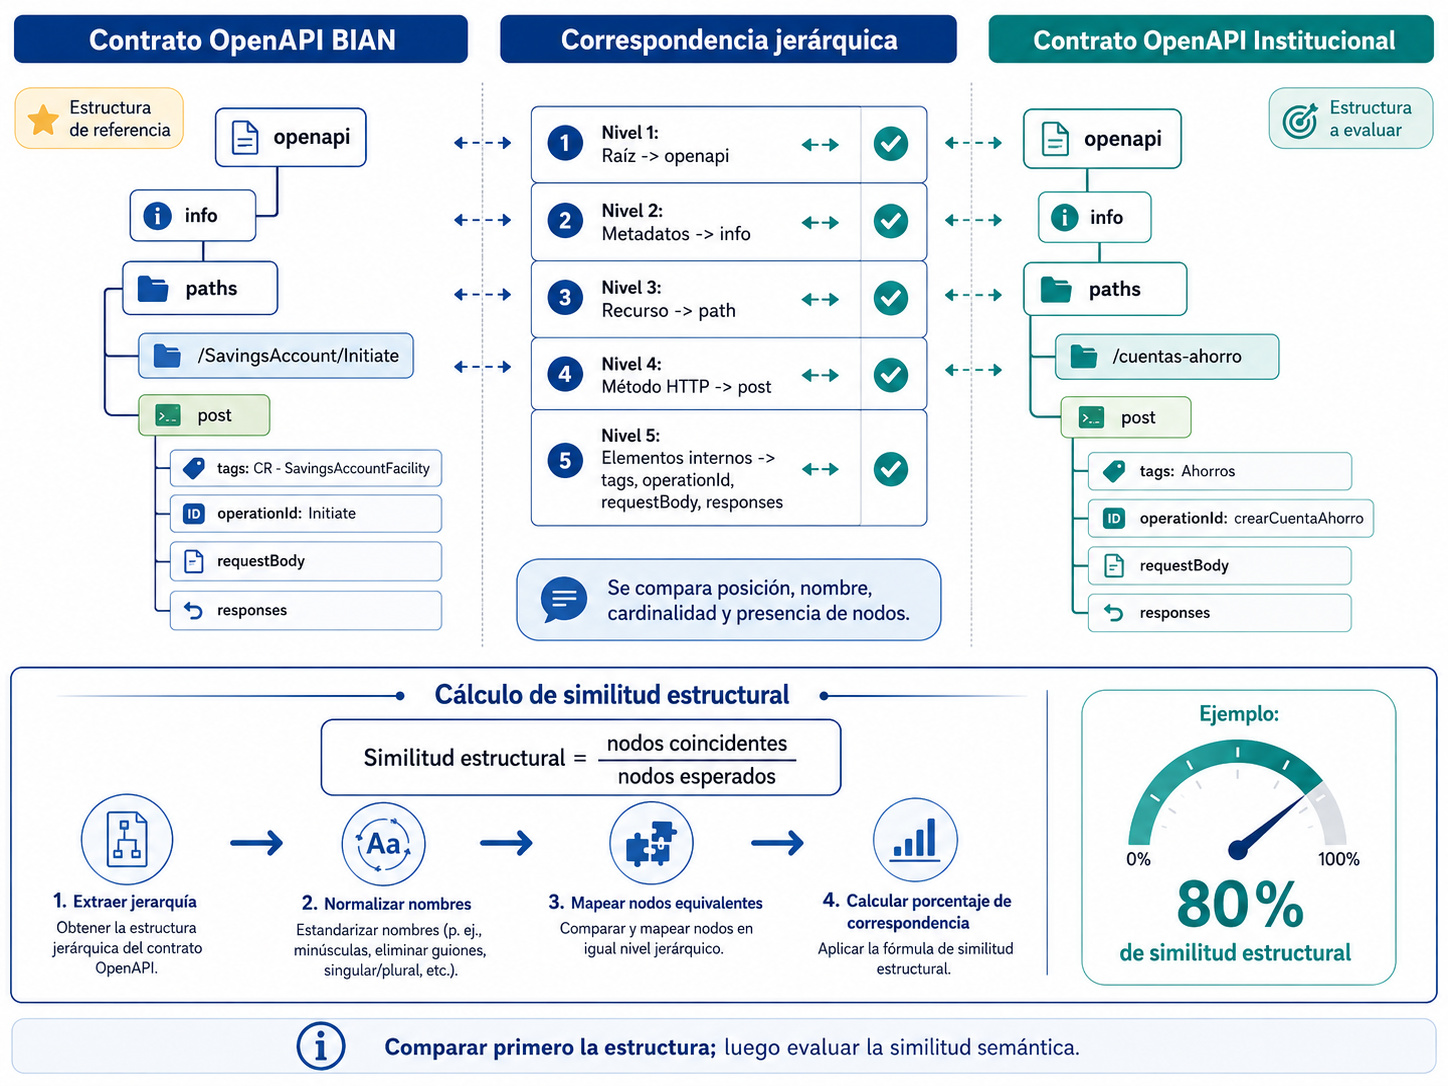
\includegraphics[width=0.92\textwidth]{Figura_07_StructuralScore}
  \caption{Correspondencia que entra en el StructuralScore}
  \label{fig:estructural}
\end{figure} El greedy asigna cada operación una sola vez. La operación OFB sin par entra como 0. E es la media de $e_{\mathrm{pair}}$ sobre todas las operaciones OFB.

\subsection{SemanticScore}

S v0, solo en los pares, es la media de dos cosas: el Jaccard de los tokens y el coseno TF-IDF. Sin GPU. El texto de OFB está en portugués y el de BIAN en inglés. Por eso el S léxico se queda cerca de cero.

S v1 usa \texttt{sentence-transformers/paraphrase-multilingual-MiniLM-L12-v2}, ya entrenado, sin fine-tuning. El vector se normaliza y el coseno es el producto punto. S v1 es la media de esos cosenos sobre los mismos pares. Los cortes 0,45 / 0,55 / 0,65 se guardan como sensibilidad. No recortan el S oficial.

\subsection{CoverageScore y AlignmentScore}

C es la fracción de tags \texttt{CR} y \texttt{BQ} del Service Domain que recibieron al menos un par.

\begin{figure}[ht]
  \centering
  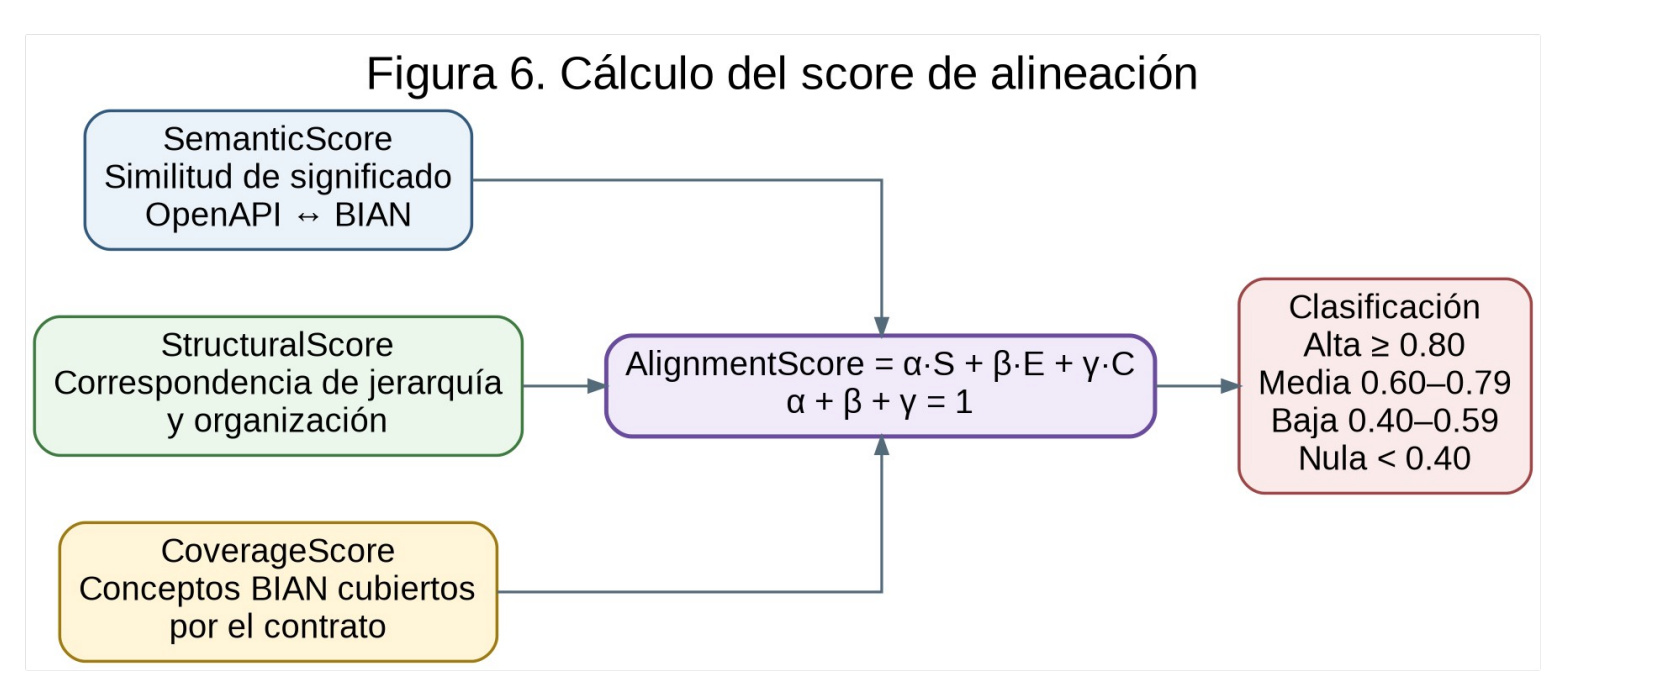
\includegraphics[width=0.85\textwidth]{Figura_03_AlignmentScore}
  \caption{S, E y C entran en el AlignmentScore}
  \label{fig:score}
\end{figure}

AlignmentScore oficial $= (S + E + C) / 3$. La sensibilidad, sin cambiar el número oficial, usa $(0{,}50,\ 0{,}30,\ 0{,}20)$ y $(0{,}20,\ 0{,}50,\ 0{,}30)$.

\begin{table}[ht]
  \centering
  \caption{Niveles del AlignmentScore}
  \label{tab:niveles}
  \begin{tabular}{@{}ll@{}}
    \toprule
    Nivel & Corte \\
    \midrule
    Alta & 0,80 o más \\
    Media & 0,60--0,79 \\
    Baja & 0,40--0,59 \\
    Nula & menor que 0,40 \\
    \bottomrule
  \end{tabular}
\end{table}

\section{Análisis de los datos y resultados}

S de la tabla es MiniLM. E y C son los del matching v0. El detalle está en el archivo \path{results/matching_s1/COMPARACION_V0_V1.md} del piloto.

\begin{table}[ht]
  \centering
  \caption{Scores preliminares de I1 a I6}
  \label{tab:scores}
  \small
  \begin{tabular}{@{}lrrrrrrl@{}}
    \toprule
    ID & S léxico & S MiniLM & E & C & Score v0 & Score v1 & Nivel \\
    \midrule
    I1 & 0,01 & 0,56 & 0,35 & 0,40 & 0,26 & 0,44 & Nula $\to$ Baja \\
    I2 & 0,01 & 0,53 & 0,47 & 0,50 & 0,33 & 0,50 & Nula $\to$ Baja \\
    I3a & 0,00 & 0,45 & 0,56 & 0,20 & 0,25 & 0,41 & Nula $\to$ Baja \\
    I3b & 0,00 & 0,46 & 0,56 & 0,20 & 0,25 & 0,41 & Nula $\to$ Baja \\
    I4 & 0,00 & 0,52 & 0,29 & 0,25 & 0,18 & 0,35 & Nula $\to$ Nula \\
    I5 & 0,03 & 0,59 & 0,32 & 0,50 & 0,28 & 0,47 & Nula $\to$ Baja \\
    I6 & 0,00 & 0,00 & 0,00 & 0,00 & 0,00 & 0,00 & Nula $\to$ Nula \\
    \bottomrule
  \end{tabular}
\end{table}

Pares que armó el greedy, sobre operaciones OFB: I1 4/6, I2 5/6, I3a 2/2, I3b 2/2, I4 3/6, I5 4/7, I6 0/8.

Los dos juegos de pesos, $(0{,}50,\ 0{,}30,\ 0{,}20)$ y $(0{,}20,\ 0{,}50,\ 0{,}30)$, dejan el nivel oficial igual en las siete instancias. En I4 el peso mayor sobre S da 0,399 y sigue en Nula. El S de la tabla es la media y no se recorta. Si pusiéramos en cero los pares con coseno bajo 0,45, I3a bajaría a 0,340 e I3b a 0,341, de Baja a Nula. Con el corte 0,55, I1 bajaría a 0,394, también Nula. Esos cortes son una bandera. No cambian el score de la tabla.

\begin{figure}[ht]
  \centering
  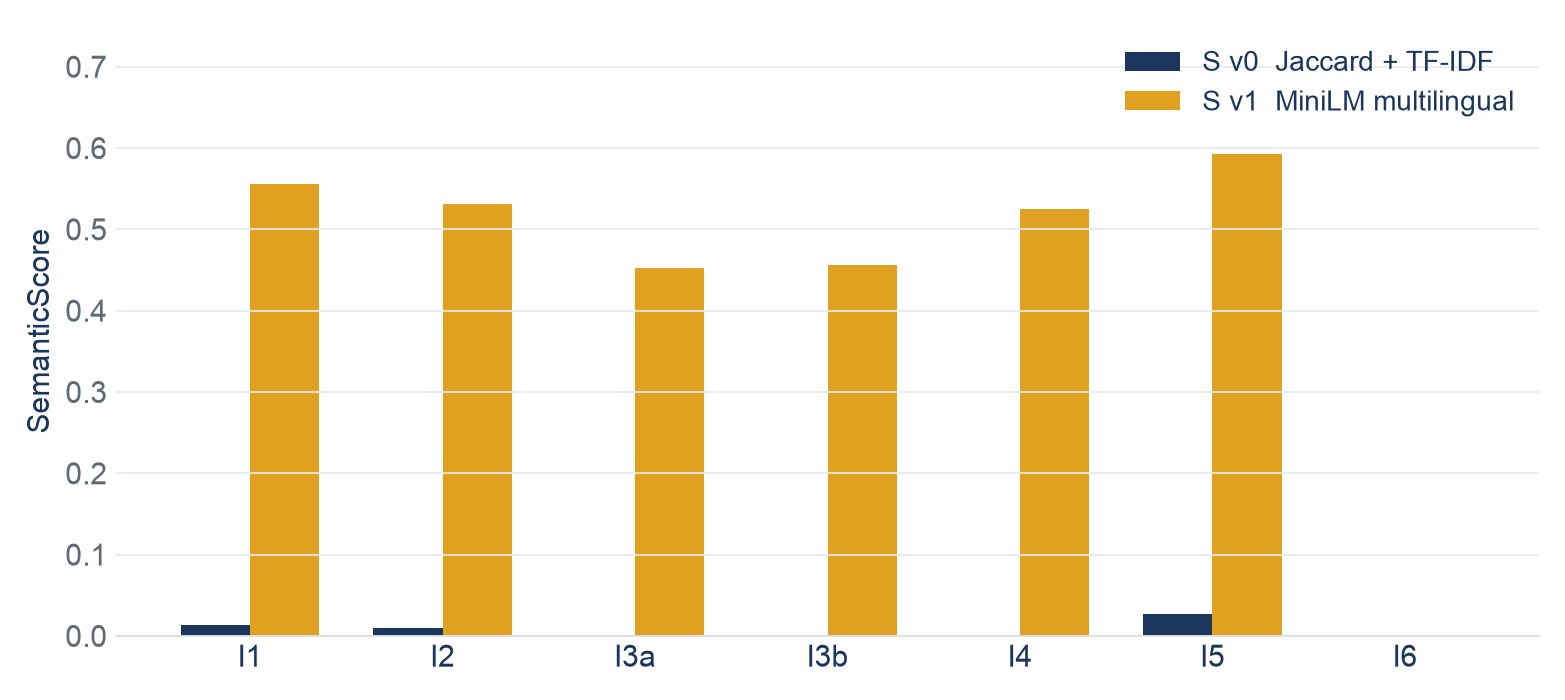
\includegraphics[width=0.88\textwidth]{grafico-semantico}
  \caption{SemanticScore. El léxico queda en el piso. MiniLM sube I1 a I5 y deja I6 en cero}
  \label{fig:semantico}
\end{figure}

\begin{figure}[ht]
  \centering
  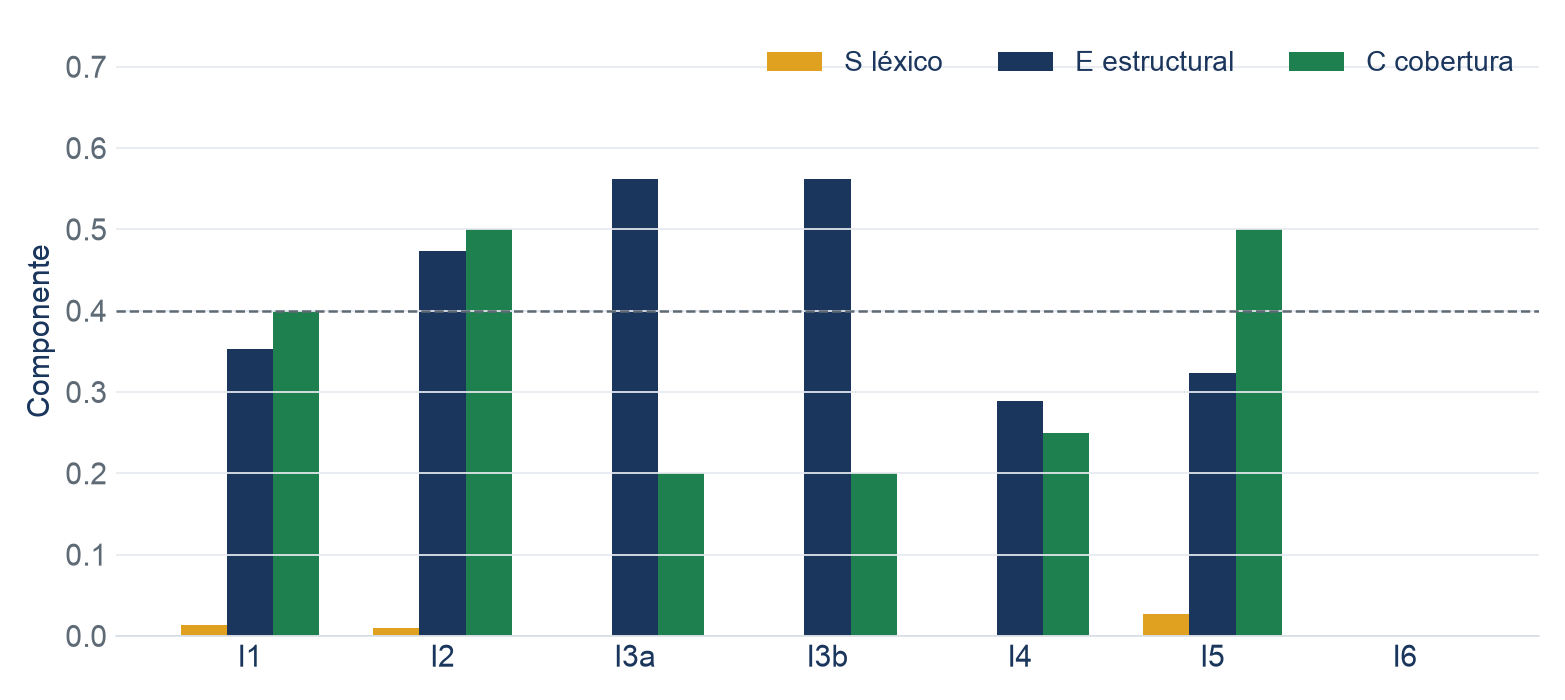
\includegraphics[width=0.88\textwidth]{grafico-sec}
  \caption{S léxico, E y C del matching v0. La línea punteada es 0,40}
  \label{fig:sec}
\end{figure}

\begin{figure}[ht]
  \centering
  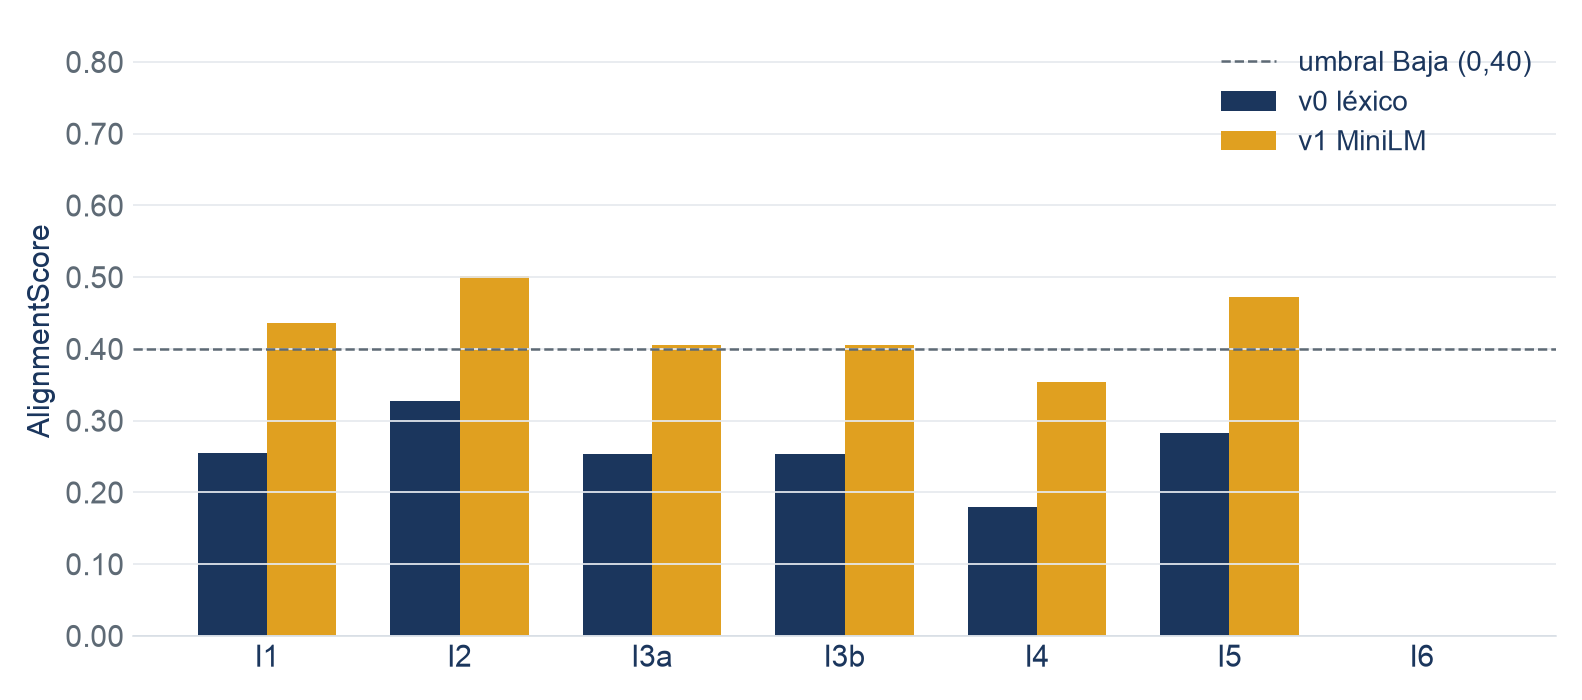
\includegraphics[width=0.88\textwidth]{grafico-alignment}
  \caption{AlignmentScore v0 y v1. I6 no tiene barra. La línea punteada es el corte de Baja}
  \label{fig:alignment}
\end{figure}

El catálogo extra (préstamos, tarjetas, inversiones) no entra en $n = 7$. El gráfico siguiente es el score v0, el léxico, no el MiniLM.

\begin{figure}[ht]
  \centering
  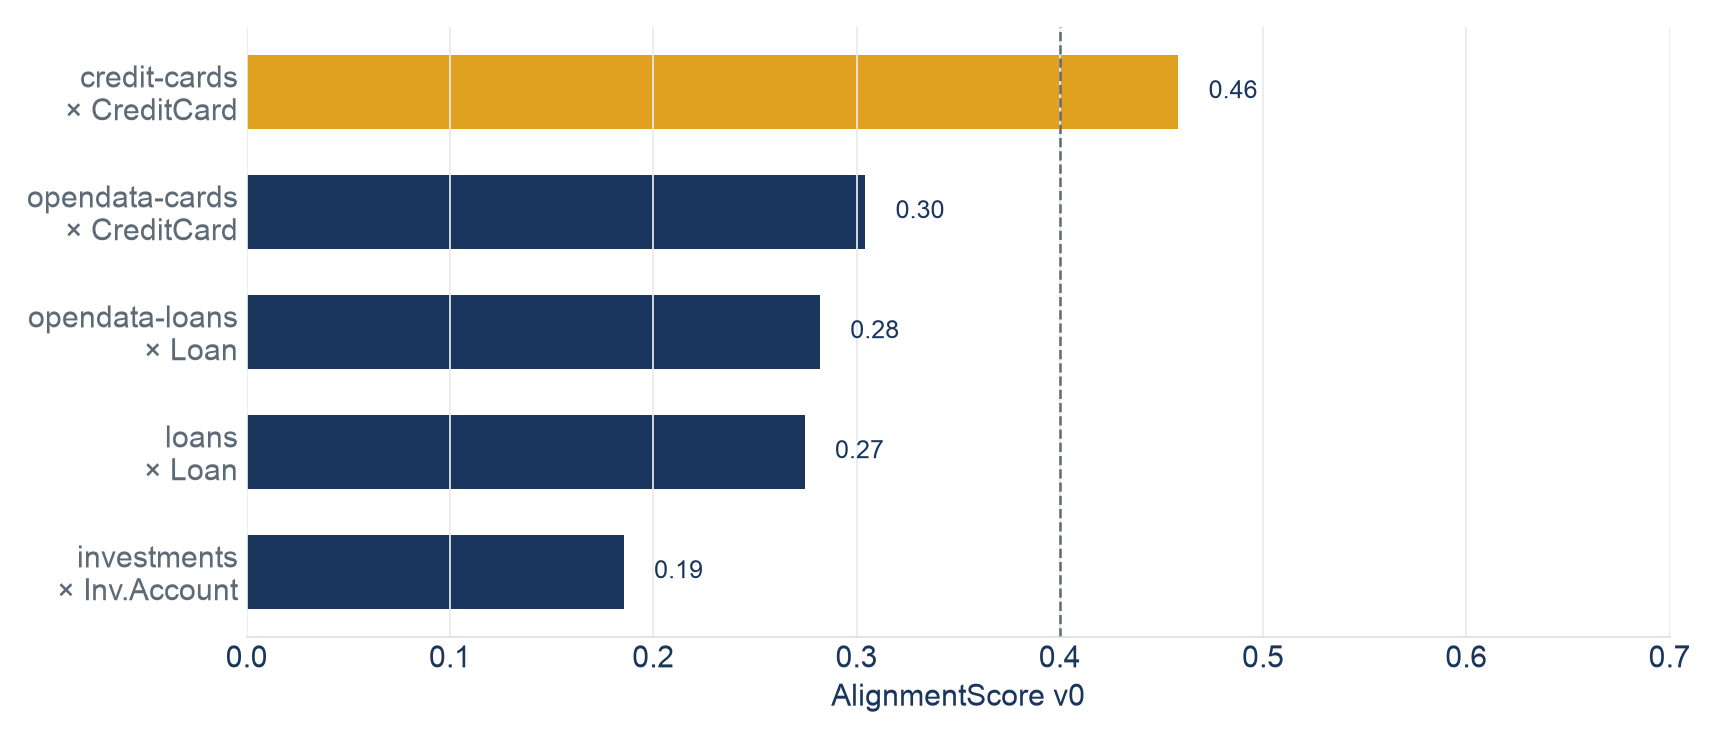
\includegraphics[width=0.82\textwidth]{grafico-catalogo}
  \caption{Catálogo v0, fuera de la muestra oficial. Solo credit-cards pasa de 0,40, y es el score léxico}
  \label{fig:catalogo}
\end{figure}

Nadie llega a Alta. Nadie llega a Media. Cinco instancias pasan de Nula a Baja cuando S deja de ser léxico. I4 se queda en Nula: S sube a 0,52, y E (0,29) con C (0,25) bajan la media a 0,35. I6 se queda en cero. No hubo par. El control negativo no inventó una correspondencia.

\section{Discusión e interpretación de los resultados}

El S léxico entre 0,00 y 0,03 no dice que las cuentas no se parezcan a Savings Account. Dice que \texttt{conta} y \texttt{SavingsAccountFacility} no comparten tokens. MiniLM, entrenado en varios idiomas y sin ajuste nuestro, sube S a la banda 0,45--0,59 en I1--I5 y lo deja en 0 en I6. El léxico es el piso. MiniLM es el S que reportamos en esta corrida.

El puntaje E no exige el mismo verbo. Si los dos son de lectura, o los dos de escritura, esa pieza vale 0,5. Si exigiéramos el verbo idéntico en el puntaje, OFB (casi todo GET) contra BIAN (casi todo PUT de ciclo de vida) caería por una convención de interfaz. Aun así E queda bajo en pagos: I4 en 0,29 e I5 en 0,32. De 6 y 7 operaciones OFB, el greedy sostiene 3 y 4 pares. Las que sobran entran como 0 en la media.

C cuenta otra cosa: cuántos tags \texttt{CR} y \texttt{BQ} del dominio recibieron par. En opendata-accounts, C $= 0{,}20$. El YAML abierto no cubre el desglose de behaviors de Savings Account.

En I1 el greedy arma cuatro pares de seis. \texttt{GET /accounts} cae en \texttt{Retrieve} (coseno 0,57), sobre Savings Account Facility. \texttt{GET /accounts/\{accountId\}}, que pide la identificación de la cuenta, cae en \texttt{RetrieveCharge} (0,59), una comisión. Los saldos caen en \texttt{RetrieveDeposit} (0,56). Las transacciones caen en \texttt{RetrieveInterest} (0,51). Quedan sin par \texttt{transactions-current} y \texttt{overdraft-limits}. C $= 0{,}40$ es 4 de 10 tags, y tres de esos cuatro son Charge, Interest y Deposit.

En I4, \texttt{POST /pix/payments} cae en \texttt{Initiate} (0,61). El GET de ese pago cae en \texttt{Retrieve} (0,47). El PATCH, cuyo texto es cancelar, cae en \texttt{Update} (0,49). Los tres consentimientos quedan sin par. C $= 0{,}25$ es un tag de cuatro: solo Payment Order Initiation Transaction. Compliance, Confirmation y Order Initiation no recibieron par.

I1 e I2 son el mismo \texttt{accounts} 2.4.2 contra dos dominios. Lo mismo I3a e I3b. La muestra de score es siete instancias y menos de siete contratos.

Los niveles no están calibrados. Hasta que etiquetemos match o no-match por recurso de negocio, y el asesor adjudique el desacuerdo, no hay kappa ni F1. Un verdadero positivo será un par del greedy que confirmemos. Un falso positivo, un par que rechacemos. Un falso negativo, un par nuestro que el greedy no armó.

\section{Estimación del impacto de la solución}

No estimamos VAN, TIR ni un costo evitado. No hay despliegue. Lo que el piloto ya cambia es la lectura del expediente de Open Finance Brasil: sin el encoder, las siete instancias quedan en Nula; con MiniLM, cinco pasan a Baja y el control negativo sigue en cero. Ese salto es el efecto medible de esta corrida.

El corpus nuevo cambia la pregunta, no el número. Casi todos los estándares de la tabla del corpus están en inglés, igual que BIAN. El piso léxico de 0,00 a 0,03 puede ser el portugués del YAML brasileño y no el desajuste de negocio. Hasta que el mismo procedimiento corra sobre Reino Unido, Berlin Group, STET o Australia, no se sabe cuál de las dos cosas es. Esas corridas no están en esta tabla.

\section{Amenazas a la validez}

La interna: el parser no aplana \texttt{allOf}, y el S léxico se acerca a cero porque el YAML del piloto está en portugués. Por eso guardamos el S v0 como piso y el S v1 no reabre los pares. La externa: los cortes 0,80 / 0,60 / 0,40 son convención, y siete instancias no representan crédito, ni un banco emisor, ni el resto del corpus. De constructo: un AlignmentScore medio puede esconder un esquema mal emparejado que al negocio le importa. De conclusión: el reporte lleva la instancia junto al score. La etiqueta y el F1 cierran esa lectura. Hasta que existan, el nivel es una convención. I6 en cero no es esa etiqueta.

\chapter{Conclusiones y recomendaciones}

\section{Conclusiones}

\begin{enumerate}
  \item El objeto es el contrato OpenAPI bancario. BIAN v14 es la referencia. El corpus de la tesis son los estándares que el 21 de noviembre se podían bajar sin cuenta: Open Finance Brasil, Reino Unido, Berlin Group (XS2A y openFinance), STET, PolishAPI, Chequia, Australia, Nueva Zelanda, Baréin y los YAML de Emiratos en Nebras. FDX y los PDF de otros países no entran al parser.
  \item De ese corpus, solo Open Finance Brasil está parseado. El parser firmó 296 de 296 YAML (38 del piloto y 258 dominios). No aplana \texttt{allOf}.
  \item En I1 a I6 el S léxico no pasa de 0,03. El texto del contrato está en portugués y el del dominio en inglés.
  \item Con MiniLM, sin fine-tuning, cinco instancias pasan de Nula a Baja. I4 se queda en Nula. I6 se queda en cero, que es lo que se esperaba del control negativo.
  \item Nadie llega a Alta ni a Media. Los cortes 0,80 / 0,60 / 0,40 siguen siendo una convención. No hay kappa ni F1.
  \item I1/I2 e I3a/I3b comparten YAML. No son siete contratos distintos. Esas siete instancias no autorizan a hablar por el resto del corpus.
\end{enumerate}

\section{Recomendaciones}

\begin{enumerate}
  \item Correr el mismo parser y el mismo matching sobre los estándares en inglés del corpus, con la versión fijada (en el Reino Unido, el tag \texttt{v4.0.1}, no \texttt{master}). El PDF del Berlin Group puede ir por delante del YAML. El número oficial sigue siendo el del archivo OpenAPI.
  \item No tratar como cerrada la licencia de Payments NZ ni la de Baréin. No tratar el repositorio de Nebras como el GitHub de CBUAE. No puntuar el YAML de ReBIT como si fuera el contrato de cuentas de un banco. VÚB, K\&H y los cajeros de la CNBV quedan en el inventario.
  \item Cerrar nuestro etiquetado, por separado y por recurso de negocio, y recién ahí calcular kappa y F1.
  \item Designar asesor. Hoy el desacuerdo del etiquetado no tiene quién lo adjudique.
  \item No correr todo el corpus contra los 258 dominios, ni meter el YAML de un banco emisor, hasta fijar esa referencia.
\end{enumerate}

\renewcommand{\bibname}{Referencias}
\begin{thebibliography}{99}
\addcontentsline{toc}{chapter}{Referencias}

\bibitem{Bhatia2022}
Bhatia, A. (2022).
\textit{Open banking and API-led connectivity in financial services}.
Informe de contexto sectorial.

\bibitem{Casas2021}
Casas, S., Cruz, D., Vidal, G., \& Constanzo, M. (2021).
Uses and applications of the OpenAPI/Swagger specification: A systematic mapping of the literature.
En \textit{Proceedings of the 40th International Conference of the Chilean Computer Science Society (SCCC)} (pp.~1--8). IEEE.
https://doi.org/10.1109/SCCC54552.2021.9650408

\bibitem{Chandrasekaran2022}
Chandrasekaran, K., \& Mago, V. (2022).
Evolution of semantic similarity: A survey.
\textit{ACM Computing Surveys}, \textit{55}(6), 1--36.

\bibitem{CMA2016}
Competition and Markets Authority. (2016).
\textit{Retail banking market investigation: Final report}.
CMA. Reino Unido.

\bibitem{ElBayadh2015}
El Bayadh, M., et al. (2015).
Ontology-alignment techniques: Survey and analysis.
\textit{International Journal of Computer Applications}, \textit{125}(9), 1--8.

\bibitem{Ehsan2022}
Ehsan, S., et al. (2022).
RESTful API testing methodologies: Rationale, challenges, and solution directions.
\textit{ACM Computing Surveys}, \textit{55}(4), 1--37.

\bibitem{Farzi2021}
Farzi, H. (2021).
\textit{BIAN Service Landscape and banking industry architecture}.
Documento de referencia BIAN.

\bibitem{Golmohammadi2024}
Golmohammadi, S., et al. (2024).
Testing RESTful APIs: A survey.
\textit{ACM Computing Surveys}, \textit{56}(9), 1--35.

\bibitem{He2022}
He, Y., Chen, J., Antonyrajah, D., \& Horrocks, I. (2022).
BERTMap: A BERT-based ontology alignment system.
En \textit{Proceedings of the AAAI Conference on Artificial Intelligence}, \textit{36}(5), 5684--5691.
https://doi.org/10.1609/aaai.v36i5.20510

\bibitem{Hertling2023}
Hertling, S., \& Paulheim, H. (2023).
OLaLa: Ontology matching with large language models.
En \textit{Proceedings of the 12th Knowledge Capture Conference (K-CAP '23)} (pp.~131--139). ACM.
https://doi.org/10.1145/3587259.3627571

\bibitem{Kotstein2024}
Kotstein, S., \& Decker, C. (2024).
RESTBERTa: A Transformer-based question answering approach for semantic search in Web API documentation.
\textit{Cluster Computing}, \textit{27}, 4035--4061.
https://doi.org/10.1007/s10586-023-04237-x

\bibitem{Lu2024}
Lu, Z., Delaney, D. T., \& Lillis, D. (2024).
Comparing the similarity of OpenAPI-based microservices.
En \textit{Proceedings of the 39th ACM/SIGAPP Symposium on Applied Computing (SAC '24)}. ACM.
https://doi.org/10.1145/3605098.3635963

\bibitem{MahanraRao2025}
Mahanra Rao, S., et al. (2025).
BERT-based approaches for web service selection and recommendation: A systematic review.
\textit{Expert Systems with Applications}, \textit{259}, 125123.

\bibitem{Mainas2023}
Mainas, A., et al. (2023).
Annotated OpenAPI descriptions and ontology for REST services.
\textit{Journal of Web Semantics}, \textit{78}, 100823.

\bibitem{Oberle2024}
Oberle, M., \& Bauernhansl, T. (2024).
Leveraging OpenAPI for microservice decomposition: A comparative study on features, encodings and algorithms on a real MES.
En \textit{Proceedings of the International Conference on Artificial Intelligence in Information and Communication (ICAIIC 2024)} (pp.~785--791). IEEE.
https://doi.org/10.1109/icaiic60209.2024.10463497

\bibitem{Otieno2026}
Otieno, J., \& Araka, J. (2026).
Systematic literature review: RESTful API testing using machine learning techniques.
\textit{Journal of Systems and Software}, \textit{220}, 112345.

\bibitem{Reimers2019}
Reimers, N. y Gurevych, I. (2019).
Sentence-BERT: Sentence embeddings using Siamese BERT-networks.
En \textit{Proceedings of the 2019 Conference on Empirical Methods in Natural Language Processing}.
El encoder de esta corrida es \texttt{sentence-transformers/paraphrase-multilingual-MiniLM-L12-v2}, sin ajuste sobre nuestros pares.

\bibitem{SantosCasas2025}
Santos, J., \& Casas, S. (2025).
A catalog of API Gateway metrics and its quantitative evaluation.
\textit{Future Generation Computer Systems}, \textit{152}, 1--15.

\bibitem{SantosSousa2026}
Santos Sousa, J., et al. (2026).
Survey on embedding methods applied to ontology matching.
\textit{ACM Computing Surveys}, \textit{58}(2), 1--38.

\bibitem{Schmidt2020}
Schmidt, R., \& Thiry, L. (2020).
Microservices identification strategies: A review focused on model-driven engineering and domain driven design.
\textit{Journal of Systems and Software}, \textit{170}, 110754.

\bibitem{Schneider2023}
Schneider, F., Dash, S., Bagshi, S., Mihindukulasooriya, N., \& Gliozzo, A. (2023).
NLFOA: Natural language focused ontology alignment.
En \textit{Proceedings of the 12th Knowledge Capture Conference (K-CAP '23)}. ACM.
https://doi.org/10.1145/3587259.3627560

\bibitem{Shabbir2025}
Shabbir, M., et al. (2025).
\textit{API quality assessment in industry practice}.
Informe de contexto sobre calidad de APIs.

\bibitem{Shvaiko2005}
Shvaiko, P., \& Euzenat, J. (2005).
A survey of schema-based matching approaches.
\textit{Journal on Data Semantics}, \textit{4}, 36--71.

\bibitem{Tanveer2025}
Tanveer, A., et al. (2025).
Towards secure APIs: A survey on RESTful API vulnerability detection.
\textit{Computers \& Security}, \textit{142}, 103891.

\bibitem{UKTreasuryTSB2018}
House of Commons Treasury Committee. (2018).
\textit{IT failure at TSB} (Ninth Report of Session 2017--19, HC 960).
House of Commons. Reino Unido.

\bibitem{Vitorino2025}
Vitorino, J., et al. (2025).
Constrained adversarial learning for automated software testing: A literature review.
\textit{Information and Software Technology}, \textit{175}, 107512.

\bibitem{ofb}
Open Finance Brasil. (s.\ f.). \textit{openapi}. GitHub.
\url{https://github.com/OpenBanking-Brasil/openapi}

\bibitem{bian}
Banking Industry Architecture Network. (s.\ f.). \textit{public}, release 14.0.0.
\url{https://github.com/bian-official/public}

\bibitem{piloto}
Mancilla Antay, A. y Paitan Cano, D. J. (2026). \textit{piloto-bank-api-bian} (commit \texttt{12c1c04}).
\url{https://github.com/denniskano/piloto-bank-api-bian}

\end{thebibliography}

\appendix
\renewcommand{\thesection}{\thechapter.\arabic{section}}
\chapter{Bitácora de la corrida}
\label{anexo:bitacora}

\begin{table}[ht]
  \centering
  \caption{Bitácora}
  \label{tab:bitacora}
  \small
  \begin{tabular}{@{}p{0.18\textwidth}p{0.36\textwidth}p{0.36\textwidth}@{}}
    \toprule
    Fecha & Qué pasó & Dónde queda \\
    \midrule
    6 nov 2026 & Parser, firma 296/296, matching v0 y MiniLM sobre I1--I6. & \texttt{oe1\_firma.json}. El commit de esa corrida, cuando el piloto aún estaba en el repositorio del curso, es \texttt{ec2b2ad}. \\
    21 nov 2026 & El piloto pasa a su repositorio. El README queda con la arquitectura y los modelos. Los scores no se recalcularon. & \url{https://github.com/denniskano/piloto-bank-api-bian}, commit \texttt{12c1c04}. \\
    21 nov 2026 & Este borrador. & \url{https://github.com/denniskano/tesis-bank-api-bian} \\
    \bottomrule
  \end{tabular}
\end{table}

Dificultades que ya vimos: el techo léxico portugués--inglés; el parser que no aplana \texttt{allOf}; I1/I2 e I3a/I3b que no son independientes; los umbrales sin etiquetas; el asesor todavía sin designar.

\chapter{Cómo repetir la corrida}
\label{anexo:repro}

Otra persona clona el piloto, no este repositorio.

\begin{lstlisting}
git clone https://github.com/denniskano/piloto-bank-api-bian.git
cd piloto-bank-api-bian
git checkout 12c1c04
python3 -m venv .venv
source .venv/bin/activate
pip install -e .
python -m ofb_bian.procesar_openapi
python -m ofb_bian.matching_v0
python -m ofb_bian.matching_s1
\end{lstlisting}

Python 3.11 o superior. En \path{pyproject.toml} el mínimo es PyYAML 6, sentence-transformers 3 y numpy 1.26. La primera vez, \path{matching_s1} descarga MiniLM desde Hugging Face. El resultado comparable es la tabla de \path{results/matching_s1/COMPARACION_V0_V1.md}. El orden no se salta: \path{matching_v0} lee los CSV del parser, y esos CSV no están en GitHub.

\chapter{Cadena de búsqueda y criterios de selección}
\label{anexo:busqueda}

\section{Bases, período e idioma}

IEEE Xplore, ACM Digital Library, Scopus / ScienceDirect, y Google Scholar como complemento. El período es 2005--2026, con énfasis en 2015--2026 para OpenAPI 3.x y el Service Landscape de BIAN. El idioma de búsqueda es el inglés. Se dejó entrar el español cuando el mapeo es de OpenAPI, como Casas et al.\ \cite{Casas2021}.

\section{Cadenas}

\begin{description}
  \item[OpenAPI.] {\small\raggedright \texttt{("OpenAPI" OR "Swagger" OR "OpenAPI Specification")} \texttt{AND ("REST" OR "RESTful") AND ("API" OR "web service")}\par}
  \item[Alineación.] {\small\raggedright \texttt{("schema matching" OR "ontology alignment"} \texttt{OR "semantic similarity" OR "structural alignment")} \texttt{AND ("OpenAPI" OR "API specification")}\par}
  \item[Banca.] {\small\raggedright \texttt{("BIAN" OR "banking architecture"} \texttt{OR "financial services" OR "open banking")} \texttt{AND ("API" OR "service domain" OR "enterprise architecture")}\par}
\end{description}

\section{Inclusión y exclusión}

Entra un survey, un mapeo o una revisión con método explícito, sobre OpenAPI, matching, ontologías, arquitectura bancaria o calidad de APIs REST, con el PDF disponible, y con algo que decir sobre el vacío OpenAPI--BIAN o sobre S, E o C.

No entra un poster ni un preprint sin revisión, salvo como contexto. No entra un trabajo que solo mide latencia de un gateway. Si el mismo estudio está en conferencia y en journal, nos quedamos con el más completo. No entra un paper cuya técnica no se puede atar al contrato OpenAPI bancario.

La tabla del anexo siguiente tiene los 20 registros de los ejes E1 a E6. Los seis de 2022--2024 (He, Schneider, Hertling, Lu, Kotstein, Oberle) van en E3 y en E4.

\chapter{Matriz de papers}
\label{anexo:papers}

\begin{longtable}{@{}p{0.08\textwidth}p{0.08\textwidth}p{0.22\textwidth}p{0.16\textwidth}p{0.34\textwidth}@{}}
\caption{Veinte papers del estado del arte} \label{tab:anexo-b} \\
\toprule
ID & Eje & Cita & Tipo & Título \\
\midrule
\endfirsthead
\multicolumn{5}{l}{\textit{(continúa)}} \\
\midrule
ID & Eje & Cita & Tipo & Título \\
\midrule
\endhead
\midrule
\multicolumn{5}{r}{\textit{(continúa)}} \\
\endfoot
\bottomrule
\endlastfoot
E1-01 & E1 & Casas et al., 2021 & mapeo & Uses and applications of the OpenAPI/Swagger specification \\
E1-02 & E1 & Mainas et al., 2023 & artículo & Annotated OpenAPI descriptions and ontology for REST services \\
E1-03 & E1 & Santos y Casas, 2025 & artículo & A catalog of API Gateway metrics and its quantitative evaluation \\
E2-01 & E2 & Shvaiko y Euzenat, 2005 & survey & A survey of schema-based matching approaches \\
E3-01 & E3 & El Bayadh et al., 2015 & survey & Ontology-alignment techniques: survey and analysis \\
E3-02 & E3 & Chandrasekaran y Mago, 2022 & survey & Evolution of semantic similarity: a survey \\
E3-03 & E3 & Santos Sousa et al., 2026 & survey & Survey on embedding methods applied to ontology matching \\
E3-04 & E3 & He et al., 2022 & artículo & BERTMap: a BERT-based ontology alignment system \\
E3-05 & E3 & Schneider et al., 2023 & artículo & NLFOA: natural language focused ontology alignment \\
E3-06 & E3 & Hertling y Paulheim, 2023 & artículo & OLaLa: ontology matching with large language models \\
E4-01 & E4 & Schmidt y Thiry, 2020 & revisión & Microservices identification strategies \\
E4-02 & E4 & Lu et al., 2024 & artículo & Comparing the similarity of OpenAPI-based microservices \\
E4-03 & E4 & Kotstein y Decker, 2024 & artículo & RESTBERTa: a transformer-based question answering approach for semantic search in Web API documentation \\
E4-04 & E4 & Oberle y Bauernhansl, 2024 & artículo & Leveraging OpenAPI for microservice decomposition \\
E5-01 & E5 & Ehsan et al., 2022 & survey & RESTful API testing methodologies \\
E5-02 & E5 & Golmohammadi et al., 2024 & survey & Testing RESTful APIs: a survey \\
E5-03 & E5 & Otieno y Araka, 2026 & revisión & RESTful API testing using machine learning techniques \\
E5-04 & E5 & Tanveer et al., 2025 & survey & Towards secure APIs \\
E5-05 & E5 & Vitorino et al., 2025 & revisión & Constrained adversarial learning for automated software testing \\
E6-01 & E6 & Mahanra Rao et al., 2025 & revisión & BERT-based approaches for web service selection \\
\end{longtable}

E1 es OpenAPI como estándar. E2, matching estructural. E3, similitud y ontologías. E4, microservicios e interfaces. E5, testing, y queda al borde. E6, selección de servicios, y también queda al borde.

\chapter{Matriz de consistencia}
\label{anexo:consistencia}

La matriz del grupo tiene diez columnas. En el borrador anterior se había quedado en cuatro. Aquí va completa, en horizontal, con las cinco fases. La Fase 1 fija el diseño. El prototipo y las siete instancias entran. La corrida de todo el corpus contra los 258 dominios no entra.

La situación real (TSB, los nueve bancos, los YAML públicos) no es una fila. La situación subyacente son las dos jerarquías, el contrato y el Service Domain.

El problema tecnológico: no existe un método reproducible que cuantifique en qué medida un contrato OpenAPI bancario se alinea con un Service Domain BIAN y bajo qué tipologías se desalinea.

El objetivo general: diseñar el modelo que calcula S, E, C y el AlignmentScore. Esta tesis entrega el modelo, el prototipo y el piloto de siete instancias. El objetivo de más arriba, el del sector, es que un equipo pueda leer esa coherencia antes del despliegue. No lo implementamos en un banco.

\begin{landscape}
\scriptsize
\setlength{\tabcolsep}{2pt}
\setlength{\LTleft}{0pt}
\setlength{\LTright}{0pt}
\begin{longtable}{@{}>{\raggedright\arraybackslash}p{2.15cm}>{\raggedright\arraybackslash}p{2.45cm}>{\raggedright\arraybackslash}p{2.45cm}>{\raggedright\arraybackslash}p{2.45cm}>{\raggedright\arraybackslash}p{1.7cm}>{\raggedright\arraybackslash}p{2.55cm}>{\raggedright\arraybackslash}p{2.15cm}>{\raggedright\arraybackslash}p{2.45cm}>{\raggedright\arraybackslash}p{2.55cm}>{\raggedright\arraybackslash}p{2.55cm}@{}}
\caption{Matriz de consistencia} \label{tab:consistencia} \\
\toprule
Fase & Problema & Objetivo & Producto & Factor & Estados del factor & Ratio & Hipótesis & Indicadores & Control \\
\midrule
\endfirsthead
\multicolumn{10}{l}{\textit{(continúa)}} \\
\midrule
Fase & Problema & Objetivo & Producto & Factor & Estados del factor & Ratio & Hipótesis & Indicadores & Control \\
\midrule
\endhead
\midrule
\multicolumn{10}{r}{\textit{(continúa)}} \\
\endfoot
\bottomrule
\endlastfoot
1. Diseño &
No hay un método reproducible que cuantifique la alineación de un contrato OpenAPI bancario con un Service Domain, ni las tipologías. No es el síntoma del sector. &
Definir entradas, S, E, C, la fórmula y los niveles. &
El modelo: adquirir, normalizar, calcular S, E y C, y el AlignmentScore. El prototipo lo corre. &
No aplica &
No aplica &
Si el diseño alcanza &
Un modelo por componentes S, E y C deja un score repetible. &
Etapas definidas, traza de la entrada a la salida, cortes de nivel escritos. &
OpenAPI bancario contra Service Domains BIAN. El prototipo ejecuta el procedimiento. Fuera: el despliegue y la corrida 38$\times$258. Cortes 0,80 / 0,60 / 0,40, convención hasta que haya etiquetas. \\
2. OE1 &
El contrato y el dominio no se comparan directo: uno es REST y el otro es negocio (P1, P2). &
Pasar los dos a una tabla común. &
Filas versionadas: paths, operaciones, schemas, behaviors y business objects. &
Representación &
Elegida: tabla (operación, ruta, verbo, esquema, texto). Descartados: grafo y RDF. &
Completitud de la extracción &
Esa tabla habilita S, E y C. &
Elementos extraídos frente a los declarados en el YAML. Integridad de la ruta, el verbo y el texto. &
38 YAML de Open Finance Brasil y 258 dominios BIAN v14. El parser firma 296/296. El score no es ese producto. Es I1 a I6. I1 e I2 comparten el YAML de accounts. I3a e I3b comparten opendata-accounts. \\
3. OE2, P1 &
No se conocen las correspondencias de jerarquía entre el contrato y el Service Domain. &
Calcular E. &
Pares estructurales y E en $[0,1]$. &
Matching &
Greedy uno a uno. Entra si el Jaccard del nombre llega a 0,40, o el último tramo de la ruta toca el recurso, o el verbo es el mismo y el Jaccard llega a 0,25. $e_{\mathrm{pair}} = 0{,}40$ nombre $+ 0{,}25$ ruta $+ 0{,}20$ verbo $+ 0{,}15$ profundidad. El verbo suma 1 si es idéntico y 0,5 si los dos son de lectura o los dos de escritura. Sin par, la operación vale 0. &
E &
El schema matching deja un E de la correspondencia REST--dominio. &
Media de $e_{\mathrm{pair}}$ sobre las operaciones del contrato. La que no tiene par entra como 0. Número de pares del greedy. &
Los mismos archivos de la fase 2. Esos pares quedan congelados para S. I6 es el control negativo: enrollments no comparte recurso con Payment Order Initiation. \\
4. OE3, P2 &
No se sabe el parecido entre los términos del dominio y los nombres del contrato. &
Calcular S. &
S en $[0,1]$, léxico y MiniLM, por separado. &
Similitud &
Sobre los pares que congeló E. v0: (Jaccard + coseno TF-IDF) / 2. v1: coseno de paraphrase-multilingual-MiniLM-L12-v2, ya entrenado, sin fine-tuning. El par no lo arma un modelo generativo. E y C no se recalculan. &
S &
S separa un concepto alineado de uno que no lo está. &
S v0 y S v1, cada uno en $[0,1]$. Los cortes de coseno 0,45 / 0,55 / 0,65 no recortan el S oficial. &
Los mismos pares de la fase 3. OFB en portugués, BIAN en inglés. Sin ajuste y sin GPU obligatoria. \\
5. OE4, P4 &
No hay un indicador que junte S, E y la cobertura, ni una escala para leerlo. P3, las tipologías, se lee en los pares. No es un quinto score. &
Calcular C, el AlignmentScore y el nivel. La sensibilidad de los pesos ya está. Precision, recall, F1 y kappa esperan etiquetas. &
C, el score, el nivel (Alta $\geq 0{,}80$, Media 0,60--0,79, Baja 0,40--0,59, Nula menor que 0,40). F1 y kappa cuando el etiquetado cierre. &
Pesos $\alpha$, $\beta$, $\gamma$ &
Oficial: los tres valen $1/3$. Sensibilidad: $(0{,}50,\ 0{,}30,\ 0{,}20)$ y $(0{,}20,\ 0{,}50,\ 0{,}30)$. &
AlignmentScore &
La media de S, E y C se puede clasificar por nivel. &
C es tags CR/BQ con par sobre tags del dominio. Score $(S+E+C)/3$. Un verdadero positivo es un par del greedy que confirmamos. Un falso positivo, un par que rechazamos. Un falso negativo, un par nuestro que el greedy no armó. &
Los pesos oficiales son los del número que se reporta. Etiquetamos por recurso de negocio, no por el verbo. El asesor adjudica el desacuerdo. Sigue por designar. I6 en cero no es nuestra etiqueta. \\
\end{longtable}
\end{landscape}

\begin{table}[ht]
  \centering
  \caption{Trazabilidad. Las citas de capítulo son las de esta tesis, no las del plan}
  \label{tab:trazabilidad}
  \footnotesize
  \begin{tabular}{@{}p{0.28\textwidth}p{0.42\textwidth}p{0.22\textwidth}@{}}
    \toprule
    Elemento & Qué es & Dónde \\
    \midrule
    Situación real & TSB, la CMA, los YAML públicos & \S 1.1 \\
    Problema abstracto & Dos jerarquías, contrato y dominio & \S 1.2 y \S 1.3 \\
    Problema tecnológico & No hay un método que deje el número & \S 1.3 \\
    Objetivo superior & Leerlo antes del despliegue. No lo hacemos en un banco & \S 1.4 \\
    Objetivo general & S, E, C y el AlignmentScore & \S 1.4 \\
    OE1 a OE4 & Tabla, E, S, y C con el nivel & Fases 2 a 5 \\
    P1 & Correspondencia estructural, la responde OE2 & \S 1.3 \\
    P2 & Parecido de significado, lo responde OE3 & \S 1.3 \\
    P3 & Tipologías. Se leen en los pares. No hay un cuarto score & \S 1.3 \\
    P4 & El indicador por instancia & \S 1.4 y fase 5 \\
    Prototipo & Parser, greedy y MiniLM, sobre I1--I6 & Capítulo III \\
    Muestra & Siete instancias. Fuera: 38$\times$258 y el banco emisor & \S 1.8 y capítulo III \\
    Etiquetas & Kappa, precision, recall y F1. Sin número todavía & \S 1.5 \\
    \bottomrule
  \end{tabular}
\end{table}

\chapter{Operación de variables}
\label{anexo:operacion}

\begin{longtable}{@{}p{0.18\textwidth}p{0.22\textwidth}p{0.14\textwidth}p{0.22\textwidth}p{0.14\textwidth}@{}}
\caption{Cómo se mide cada ratio} \label{tab:operacion} \\
\toprule
Ratio & Definición & Escala & Cálculo & Control \\
\midrule
\endfirsthead
\multicolumn{5}{l}{\textit{(continúa)}} \\
\midrule
Ratio & Definición & Escala & Cálculo & Control \\
\midrule
\endhead
\midrule
\multicolumn{5}{r}{\textit{(continúa)}} \\
\endfoot
\bottomrule
\endlastfoot
E & Correspondencia estructural & $[0,1]$ & Media de $e_{\mathrm{pair}}$ sobre todas las operaciones del contrato. Sin par, entra 0 & Pesos 0,40 / 0,25 / 0,20 / 0,15 \\
S & Parecido de los textos emparejados & $[0,1]$ & v0: media de Jaccard y coseno TF-IDF. v1: coseno MiniLM. Solo los pares & Mismos pares. Sin fine-tuning \\
C & Tags CR/BQ del dominio con al menos un par & $[0,1]$ & Tags con par / tags del dominio & No se copian tags al YAML de origen \\
AlignmentScore & Indicador de la instancia & $[0,1]$ & $(S+E+C)/3$ & Los tres pesos suman 1 \\
Nivel & Lectura del score & 4 clases & 0,80 / 0,60 / 0,40 & Convención, hasta que haya F1 \\
Extracción & Completitud del parser & ratio & Extraídos / declarados en el YAML & Firma 296/296 en el piloto \\
\end{longtable}

Los factores ya elegidos: tabla (no grafo ni RDF); greedy uno a uno; Jaccard con TF-IDF y MiniLM; pesos iguales en el número oficial, y dos juegos de sensibilidad que no lo reemplazan.

\chapter{Diseño factorial}
\label{anexo:factorial}

El diseño factorial completo no aplica. El producto es el procedimiento y los scores, no un experimento que cruce todas las alternativas. Los factores ya tienen una configuración (anexo anterior). Lo que sí entra es la sensibilidad de los tres pesos y, cuando haya etiquetas, el F1 del emparejamiento.

\chapter{Administración del trabajo}
\label{anexo:admin}

El plazo de los datos generales es septiembre 2026 a enero 2027. El asesor sigue por designar: la última fila le reserva la revisión y no le pone un nombre.

\begin{table}[ht]
  \centering
  \caption{Cronograma}
  \label{tab:cronograma}
  \small
  \begin{tabular}{@{}clll@{}}
    \toprule
    Fase & Actividad & Cuándo & Quién \\
    \midrule
    0 & Bibliografía, cadenas de búsqueda y brecha & Sep 2026 & Alex \\
    0 & YAML del piloto y parser de los 296 contratos & Sep--oct 2026 & Jack \\
    1 & Planteamiento, objeto, justificación y clasificación & Sep--oct 2026 & Alex \\
    2 & Matching v0 de I1--I6 (E, S léxico, C) & Oct--nov 2026 & Jack \\
    3 & S con MiniLM sobre los pares congelados & Nov 2026 & Jack \\
    3 & Lectura de I1--I6, control I6 y figuras & Nov 2026 & Alex \\
    4 & Etiquetado independiente, por recurso de negocio & Dic 2026 & Ambos \\
    5 & Rúbrica, sensibilidad de pesos y F1 & Dic 2026--ene 2027 & Ambos \\
    6 & Cierre del borrador y revisión con el asesor & Ene 2027 & Ambos \\
    \bottomrule
  \end{tabular}
\end{table}

El presupuesto de licencias y de despliegue es cero soles: \LaTeX{}, Python, Zotero y Git. El acceso a IEEE y ACM sale de la matrícula. La impresión, si hace falta, no pasa de 30 soles y la pagan los dos. No hay financiamiento externo. El piloto corre en los equipos de los dos.

Alex lleva los capítulos I y II, la cadena de búsqueda, la brecha y la lectura de los niveles. Jack lleva el prototipo, los capítulos III y IV, y los anexos de operación. El corpus público, las figuras y el etiquetado son de los dos. Cada uno revisa el bloque del otro antes de cerrar el borrador.

El riesgo que ya vimos, y que el cronograma deja abierto, es el etiquetado: sin asesor no hay quien adjudique el desacuerdo, y sin ese cierre no hay kappa ni F1.



\end{document}
